\documentclass[11pt,twocolumn,a4paper]{article}
\usepackage{amsmath}
\usepackage{amssymb}
\usepackage{graphicx}
\usepackage{booktabs}
\usepackage{hyperref}
\usepackage{float}
\usepackage{geometry}
\usepackage{xcolor}
\usepackage{microtype}
\usepackage{titlesec}
\usepackage{caption}
\usepackage{abstract}
\usepackage{fancyhdr}
\usepackage{stfloats}

\setcounter{dbltopnumber}{3}
\renewcommand{\dbltopfraction}{0.95}
\renewcommand{\dbltextfraction}{0.05}

\geometry{
    a4paper,
    left=15mm,
    right=15mm,
    top=22mm,
    bottom=22mm,
    footskip=10mm
}

\hypersetup{
    colorlinks=true,
    linkcolor=blue,
    filecolor=magenta,      
    urlcolor=cyan,
    pdftitle={Modélisation Prédictive Multi-Régionale et Analyse Multicritère pour la Gestion des Géosites (Phase 2 - Fuzzy MCDSS Engine)},
    pdfpagemode=FullScreen,
}

\raggedbottom

\pagestyle{fancy}
\fancyhf{}
\fancyhead[L]{\textsf{GSMI-UM6P}}
\fancyhead[R]{\textsf{Rapport Technique Phase 2 — Analytics Multi-Régionales}}
\fancyfoot[C]{\thepage}
\renewcommand{\headrulewidth}{0.4pt}
\renewcommand{\footrulewidth}{0pt}

\titleformat{\section}{\large\bfseries\sffamily}{\thesection}{1em}{}
\titleformat{\subsection}{\normalsize\bfseries\sffamily}{\thesubsection}{1em}{}

\renewenvironment{abstract}{%
    \small\sffamily
    \noindent\textbf{Résumé}\quad
    \selectfont
}{%
    \vspace{0.4cm}
}

\begin{document}

\twocolumn[
    \begin{@twocolumnfalse}
        \begin{center}
            {
\includegraphics[width=0.45\textwidth]{../um6p_figures/um6p_gsmi_logo.png}}
        \end{center}
        \vspace{0.4cm}
        
        {\Huge\bfseries\sffamily Modélisation Prédictive Localisée par Apprentissage Automatique et Analyse Multicritère Floue (Fuzzy MCDSS) pour la Gestion Territoriale des Géosites : Évaluation Multi-Régionale Pilote (Béni Mellal-Khénifra \& Tanger-Tétouan-Al Hoceïma)\par}
        \vspace{0.6cm}
        
        {\large\textbf{EL GORRIM Mohamed}\par}
        {\small\sffamily Stagiaire de recherche en IA, Geology and Sustainable Mining Institute (GSMI), Université Mohammed VI Polytechnique (UM6P), Ben Guerir, Maroc\par}
        \vspace{0.4cm}
        {\small\sffamily\textbf{Préparé pour :} Dr. Ismail BEN AMAR, Sanae EL HARCHE et Mohamed EL OUALI\par}
        \vspace{0.6cm}
        
        \begin{abstract}
        L'évaluation macroscopique nationale de l'accessibilité des géosites (Phase 1) masque des hétérogénéités topographiques et structurelles régionales. Ce travail présente le livrable technique complet de la Phase 2, étendu à deux régions pilotes contrastées du Maroc sous la formulation d'un moteur d'Aide à la Décision Spatiale Multicritère Floue (Fuzzy MCDSS) : la région continentale du Haut et Moyen Atlas (\textbf{Béni Mellal-Khénifra}, $N=55$ géosites) et la région littorale et montagnarde du Rif (\textbf{Tanger-Tétouan-Al Hoceïma}, $N=51$ géosites). Pour corriger les biais spatiaux, nous réalisons un filtrage géographique rigoureux avec déduplication par coordonnées WGS84 et rectification des anomalies. Trois modèles d'apprentissage automatique sont évalués sous validation croisée 3-Fold Stratifiée et 5-Fold Spatiale par blocs ($22\,\text{km}$). Sur Béni Mellal-Khénifra, le modèle localisé \textbf{Random Forest (Basic)} surpasse les autres avec une exactitude spatiale de \textbf{87,27\%}, un F1-score spatial de \textbf{0,8585} et une concordance de \textbf{85,93\%} avec le modèle national flou. Sur Tanger-Tétouan-Al Hoceïma, le modèle \textbf{Random Forest (Basic)} offre également la meilleure généralisation spatiale avec une exactitude spatiale de \textbf{74,51\%}, un F1-score spatial de \textbf{0,7171} et une concordance de \textbf{89,32\%}. De plus, nous calculons trois indices multicritères ancrés dans la littérature de Brilha (2016) : Valeur Scientifique ($V_{\text{sci}}$), Vulnérabilité ($V_{\text{vuln}}$), et Potentiel Géotouristique ($V_{\text{geo}}$). Le partitionnement K-Means ($K=5$), validé empiriquement par l'inertie Elbow, le score Silhouette et l'index de Davies-Bouldin, classe les géosites en cinq profils opérationnels de gestion. L'analyse comparative met en lumière un contraste territorial fort entre la région continentale de BMK et la région rifaine de TTAH.
        \end{abstract}
        
        \noindent\textbf{Mots-clés} Apprentissage automatique localisé $\cdot$ Béni Mellal-Khénifra $\cdot$ Tanger-Tétouan-Al Hoceïma $\cdot$ Fuzzy MCDSS $\cdot$ Validation croisée spatiale $\cdot$ Clustering K-Means $\cdot$ Aménagement du territoire
        \vspace{0.8cm}
    \end{@twocolumnfalse}
]

\section{Introduction et Cadrage Territoire}
La modélisation nationale de l'accessibilité des géosites développée au cours de la Phase 1 a permis d'établir une cartographie prédictive de premier ordre pour l'ensemble du territoire marocain. Cependant, l'échelle macroscopique nationale ne permet pas de capturer fidèlement les micro-topographies et les conditions logistiques propres aux différentes provinces géomorphologiques du Maroc.

L'objectif de cette Phase 2 est de déployer et de valider un cadre d'analyse prédictive et d'aide à la décision territoriale sur deux régions pilotes représentatives sous un moteur flou MCDSS :
\begin{enumerate}
    \item \textbf{La Région de Béni Mellal-Khénifra (BMK, $N=55$ sites, 36 ancrés au territoire)} : secteur continental abritant le Géoparc M'Goun, caractérisé par des vallées karstiques, des plateaux calcaires et une forte densité de géosites paléontologiques et géomorphologiques.
    \item \textbf{La Région de Tanger-Tétouan-Al Hoceïma (TTAH, $N=51$ sites, 47 ancrés au territoire)} : secteur nordique associant la chaîne rifaine à relief escarpé et une bande littorale sous haute pression démographique et touristique.
\end{enumerate}

Ce rapport présente la méthodologie de filtrage spatial, la comparaison rigoureuse des classificateurs localisés sous validation spatiale par blocs ($22\,\text{km}$), la projection cartographique sur grilles physiques rasters, le calcul des indices multicritères de Brilha (2016), et l'analyse comparative des profils de gestion issus du clustering K-Means.

\section{Méthodologie et Préparation des Données}

\subsection{Filtrage Spatial et Pression Anthropique}
Une analyse géographique rigoureuse a révélé la présence de doublons géographiques dans la base brute. Après déduplication par coordonnées WGS84 et consolidation des variantes régionales, le corpus d'étude s'établit à 55 géosites pour Béni Mellal-Khénifra et 51 géosites pour Tanger-Tétouan-Al Hoceïma. Une erreur de coordonnées sur le géosite du Cap Malabata ($-0,0333^\circ\,\text{W}$ au lieu de $-5,7133^\circ\,\text{W}$) a également été rectifiée.

Pour modéliser la pression anthropique indirecte ($P_{\text{anthro}}$), les réseaux d'établissements urbains ont été extraits via l'API Overpass d'OpenStreetMap. La distance métrique au plus proche pôle urbain ($D_{\text{urban}}$) a été calculée en coordonnées projetées Sahara Lambert (EPSG:26191).

\subsection{Moteur d'Aide à la Décision Floue (Fuzzy MCDSS Engine)}
Pour éliminer les artéfacts de bordure liés aux seuils stricts (ex: $2\,000\,\text{m}$), nous introduisons des fonctions d'appartenance floues sigmoïdales continues $S_{\text{access}} \in [0, 1]$ :
\begin{equation}
\mu_{\text{hw}}(D_{\text{hwy}}) = \frac{1}{1 + e^{\frac{D_{\text{hwy}} - 2000}{400}}}
\end{equation}
\begin{equation}
\mu_{\text{piste}}(D_{\text{pst}}) = \frac{1}{1 + e^{\frac{D_{\text{pst}} - 1000}{250}}}
\end{equation}
\begin{equation}
\mu_{\text{slope}}(\theta) = \frac{1}{1 + e^{\frac{\theta - 20}{5}}}
\end{equation}
\begin{equation}
\mu_{\text{rugged}}(R) = \frac{1}{1 + e^{\frac{R - 200}{50}}}
\end{equation}

Le score continu d'accessibilité globale floue $S_{\text{access}}$ dérive de l'agrégation pondérée suivante :
\begin{equation}
S_{\text{access}} = \max\left(\mu_{\text{hw}}, 0.75 \cdot \mu_{\text{piste}}\right) \cdot \left(0.65 \cdot \mu_{\text{slope}} + 0.35 \cdot \mu_{\text{rugged}}\right)
\end{equation}

Les classes cibles sont attribuées de manière continue : \textbf{Facile} ($S \ge 0.50$), \textbf{Modérée} ($0.25 \le S < 0.50$), et \textbf{Difficile} ($S < 0.25$). Le Tableau \ref{tab:sample_reg} montre un extrait des données régionales indexées.

\begin{table*}[t]
    \centering
    \caption{Extrait du jeu de données des géosites régionaux étiquetés par le moteur Fuzzy MCDSS (5 enregistrements d'échantillon)}
    \label{tab:sample_reg}
    \resizebox{0.95\textwidth}{!}{%
    \begin{tabular}{lcccccccc}
        \toprule
        \textbf{Nom du Géosite} & \textbf{Région} & \textbf{Lat} & \textbf{Lon} & \textbf{Pente ($^\circ$)} & \textbf{Rugosité} & \textbf{Dist Route (m)} & \textbf{Score Flou ($S_{\text{access}}$)} & \textbf{Accessibilité} \\
        \midrule
        Source Ras El Ma & TTAH & 35.1689 & -5.2606 & 1.20 & 14.5 & 0.0 & \textbf{0.708} & Facile \\
        Glissement d'Akchour & TTAH & 35.2351 & -5.1762 & 2.10 & 22.1 & 0.0 & \textbf{0.708} & Facile \\
        Cascade Oued ElKelaa & TTAH & 35.1420 & -5.2110 & 18.50 & 145.2 & 4266.9 & \textbf{0.221} & Difficile \\
        Cascades d'Ouzoud & BMK & 32.0152 & -6.7189 & 3.40 & 31.2 & 0.0 & \textbf{0.695} & Facile \\
        Aïn Asserdoun & BMK & 32.3311 & -6.3492 & 0.90 & 12.0 & 0.0 & \textbf{0.712} & Facile \\
        \bottomrule
    \end{tabular}%
    }
\end{table*}

\subsection{Indices Multicritères (Brilha, 2016)}
Pour structurer la prise de décision en aménagement territorial, nous construisons trois indices à valeurs dans l'intervalle $[1,0; 5,0]$ basés sur Brilha (2016) :
\begin{itemize}
    \item \textbf{Valeur Scientifique ($V_{\text{sci}}$)} : combine le poids du type d'intérêt géologique et la rareté lithologique régionale.
    \item \textbf{Index de Vulnérabilité ($V_{\text{vuln}}$)} : intègre la vulnérabilité liée à la pente ($S_{\text{erosion}}$), la sensibilité du sol ($S_{\text{soil}}$), et la pression anthropique ($P_{\text{anthro}}$).
    \item \textbf{Potentiel Géotouristique ($V_{\text{geo}}$)} : combine l'attractivité visuelle et la sécurité logistique d'accès.
\end{itemize}

\subsection{Apprentissage Automatique Localisé et CV Spatiale}
Chaque région est évaluée indépendamment sur 3 algorithmes (Random Forest, XGBoost, HistGradientBoosting) sous deux schémas de validation : Stratifiée 3-Fold et GroupKFold Spatiale basé sur des blocs géographiques de $0,2^\circ \times 0,2^\circ$ ($\approx 22\,\text{km}$).

\section{Résultats et Discussion}

\subsection{Banc d'Essai des Modèles Régionaux}
Les résultats comparatifs de validation pour BMK et TTAH sont synthétisés dans le Tableau \ref{tab:regional_models} et visualisés dans les Figures \ref{fig:bmk_comp} et \ref{fig:ttah_comp}.

\begin{table*}[t]
\centering
\caption{Métriques d'évaluation hors-blocs des modèles régionaux localisés sous validation croisée spatiale par blocs (22 km $\times$ 22 km).}
\label{tab:regional_models}
\resizebox{0.95\textwidth}{!}{%
\begin{tabular}{lccccc}
\toprule
\textbf{Région Pilote \& Modèle} & \textbf{Exactitude Stratifiée} & \textbf{F1 Stratifié} & \textbf{Exactitude Spatiale} & \textbf{Spatial F1} & \textbf{Écart Fuite ($\Delta$)} \\
\midrule
\textbf{BMK — Random Forest (Basic)} & \textbf{96,36\%} & \textbf{0,9624} & \textbf{87,27\%} & \textbf{0,8585} & 0,1039 \\
BMK — XGBoost (Basic) & 96,36\% & 0,9625 & 85,45\% & 0,8414 & 0,1211 \\
BMK — HistGradientBoosting & 76,36\% & 0,6613 & 70,91\% & 0,7320 & 0,0707 \\
\midrule
\textbf{TTAH — Random Forest (Basic)} & \textbf{84,31\%} & \textbf{0,8477} & \textbf{74,51\%} & \textbf{0,7171} & 0,1306 \\
TTAH — XGBoost (Basic) & 76,47\% & 0,7575 & 68,63\% & 0,6636 & 0,0939 \\
TTAH — HistGradientBoosting & 60,78\% & 0,4596 & 49,02\% & 0,4281 & 0,0315 \\
\bottomrule
\end{tabular}%
}
\end{table*}

Sur la région de Béni Mellal-Khénifra, le modèle localisé \textbf{Random Forest (Basic)} obtient la meilleure performance spatiale avec un F1-score spatial de \textbf{0,8585} et une exactitude spatiale de \textbf{87,27\%}. Sur la région de Tanger-Tétouan-Al Hoceïma, le modèle \textbf{Random Forest (Basic)} surpasse également XGBoost et HistGradientBoosting avec un F1-score spatial de \textbf{0,7171} et une exactitude spatiale de \textbf{74,51\%}.

\begin{figure}[htbp]
    \centering
    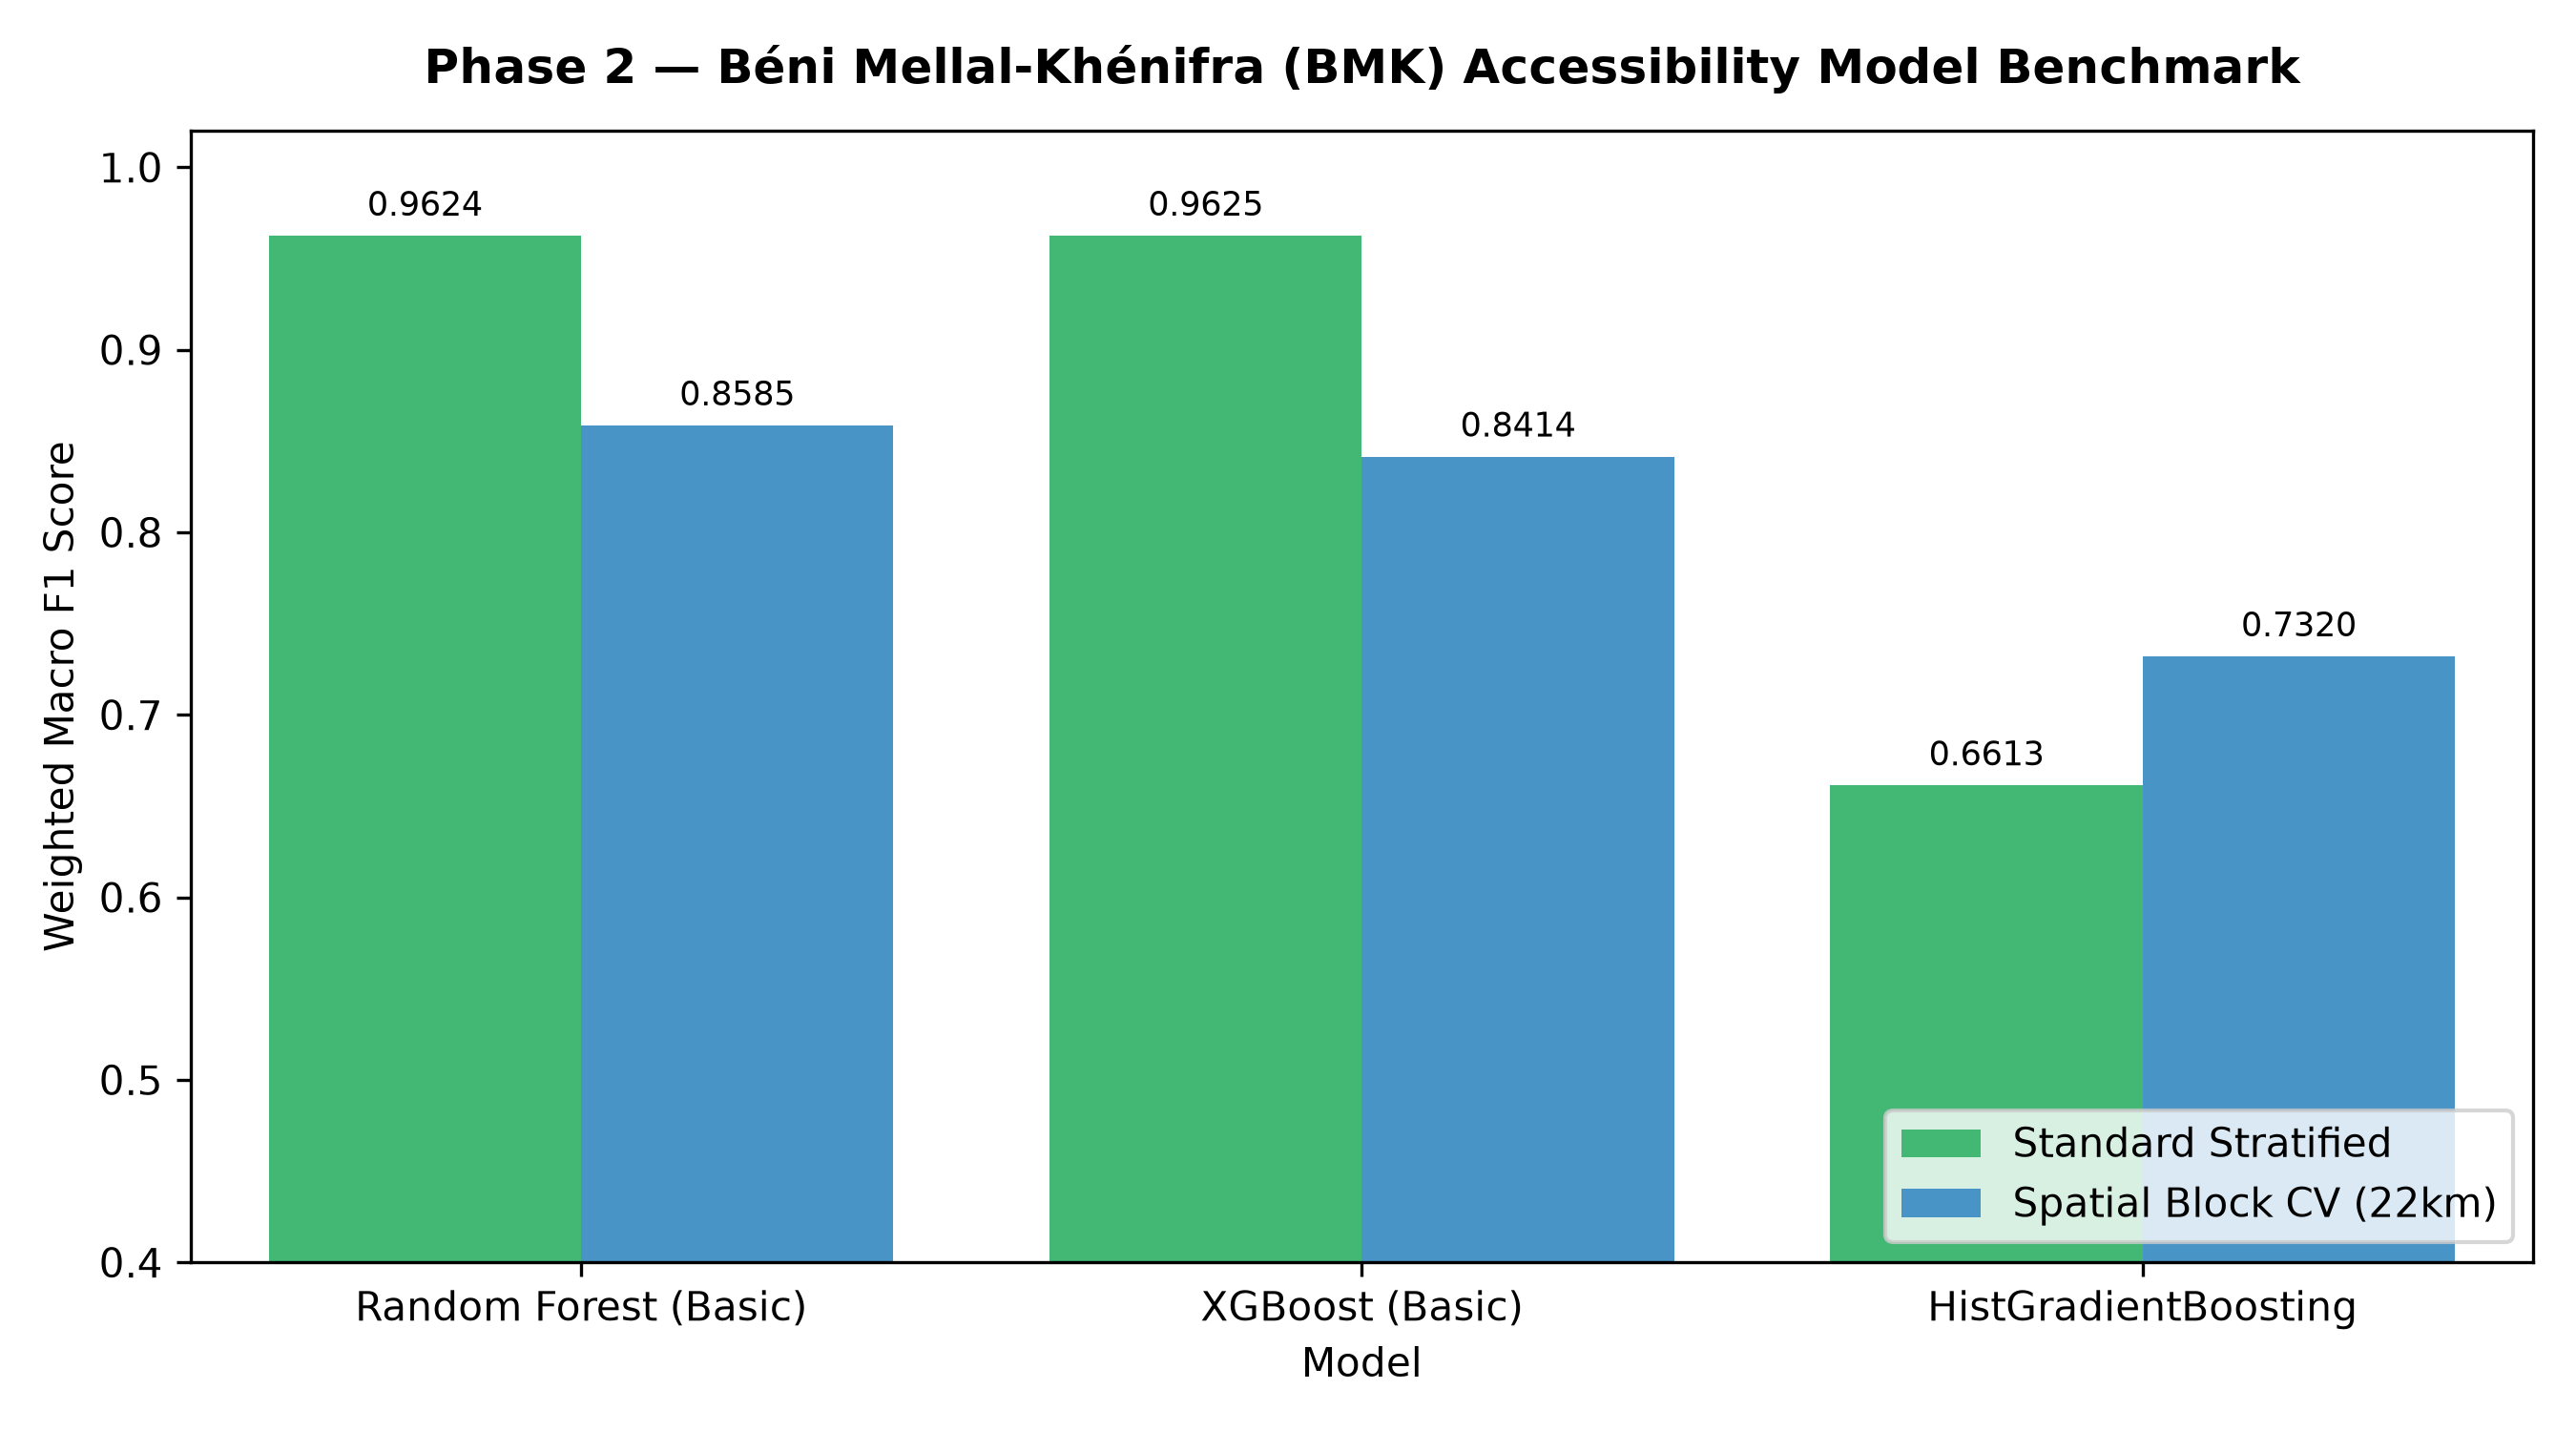
\includegraphics[width=\linewidth]{../figures/regional_model_comparison.png}
    \caption{Comparaison des modèles prédictifs pour la région Béni Mellal-Khénifra (Standard CV F1 vs Spatial Block CV F1).}
    \label{fig:bmk_comp}
\end{figure}

\begin{figure}[htbp]
    \centering
    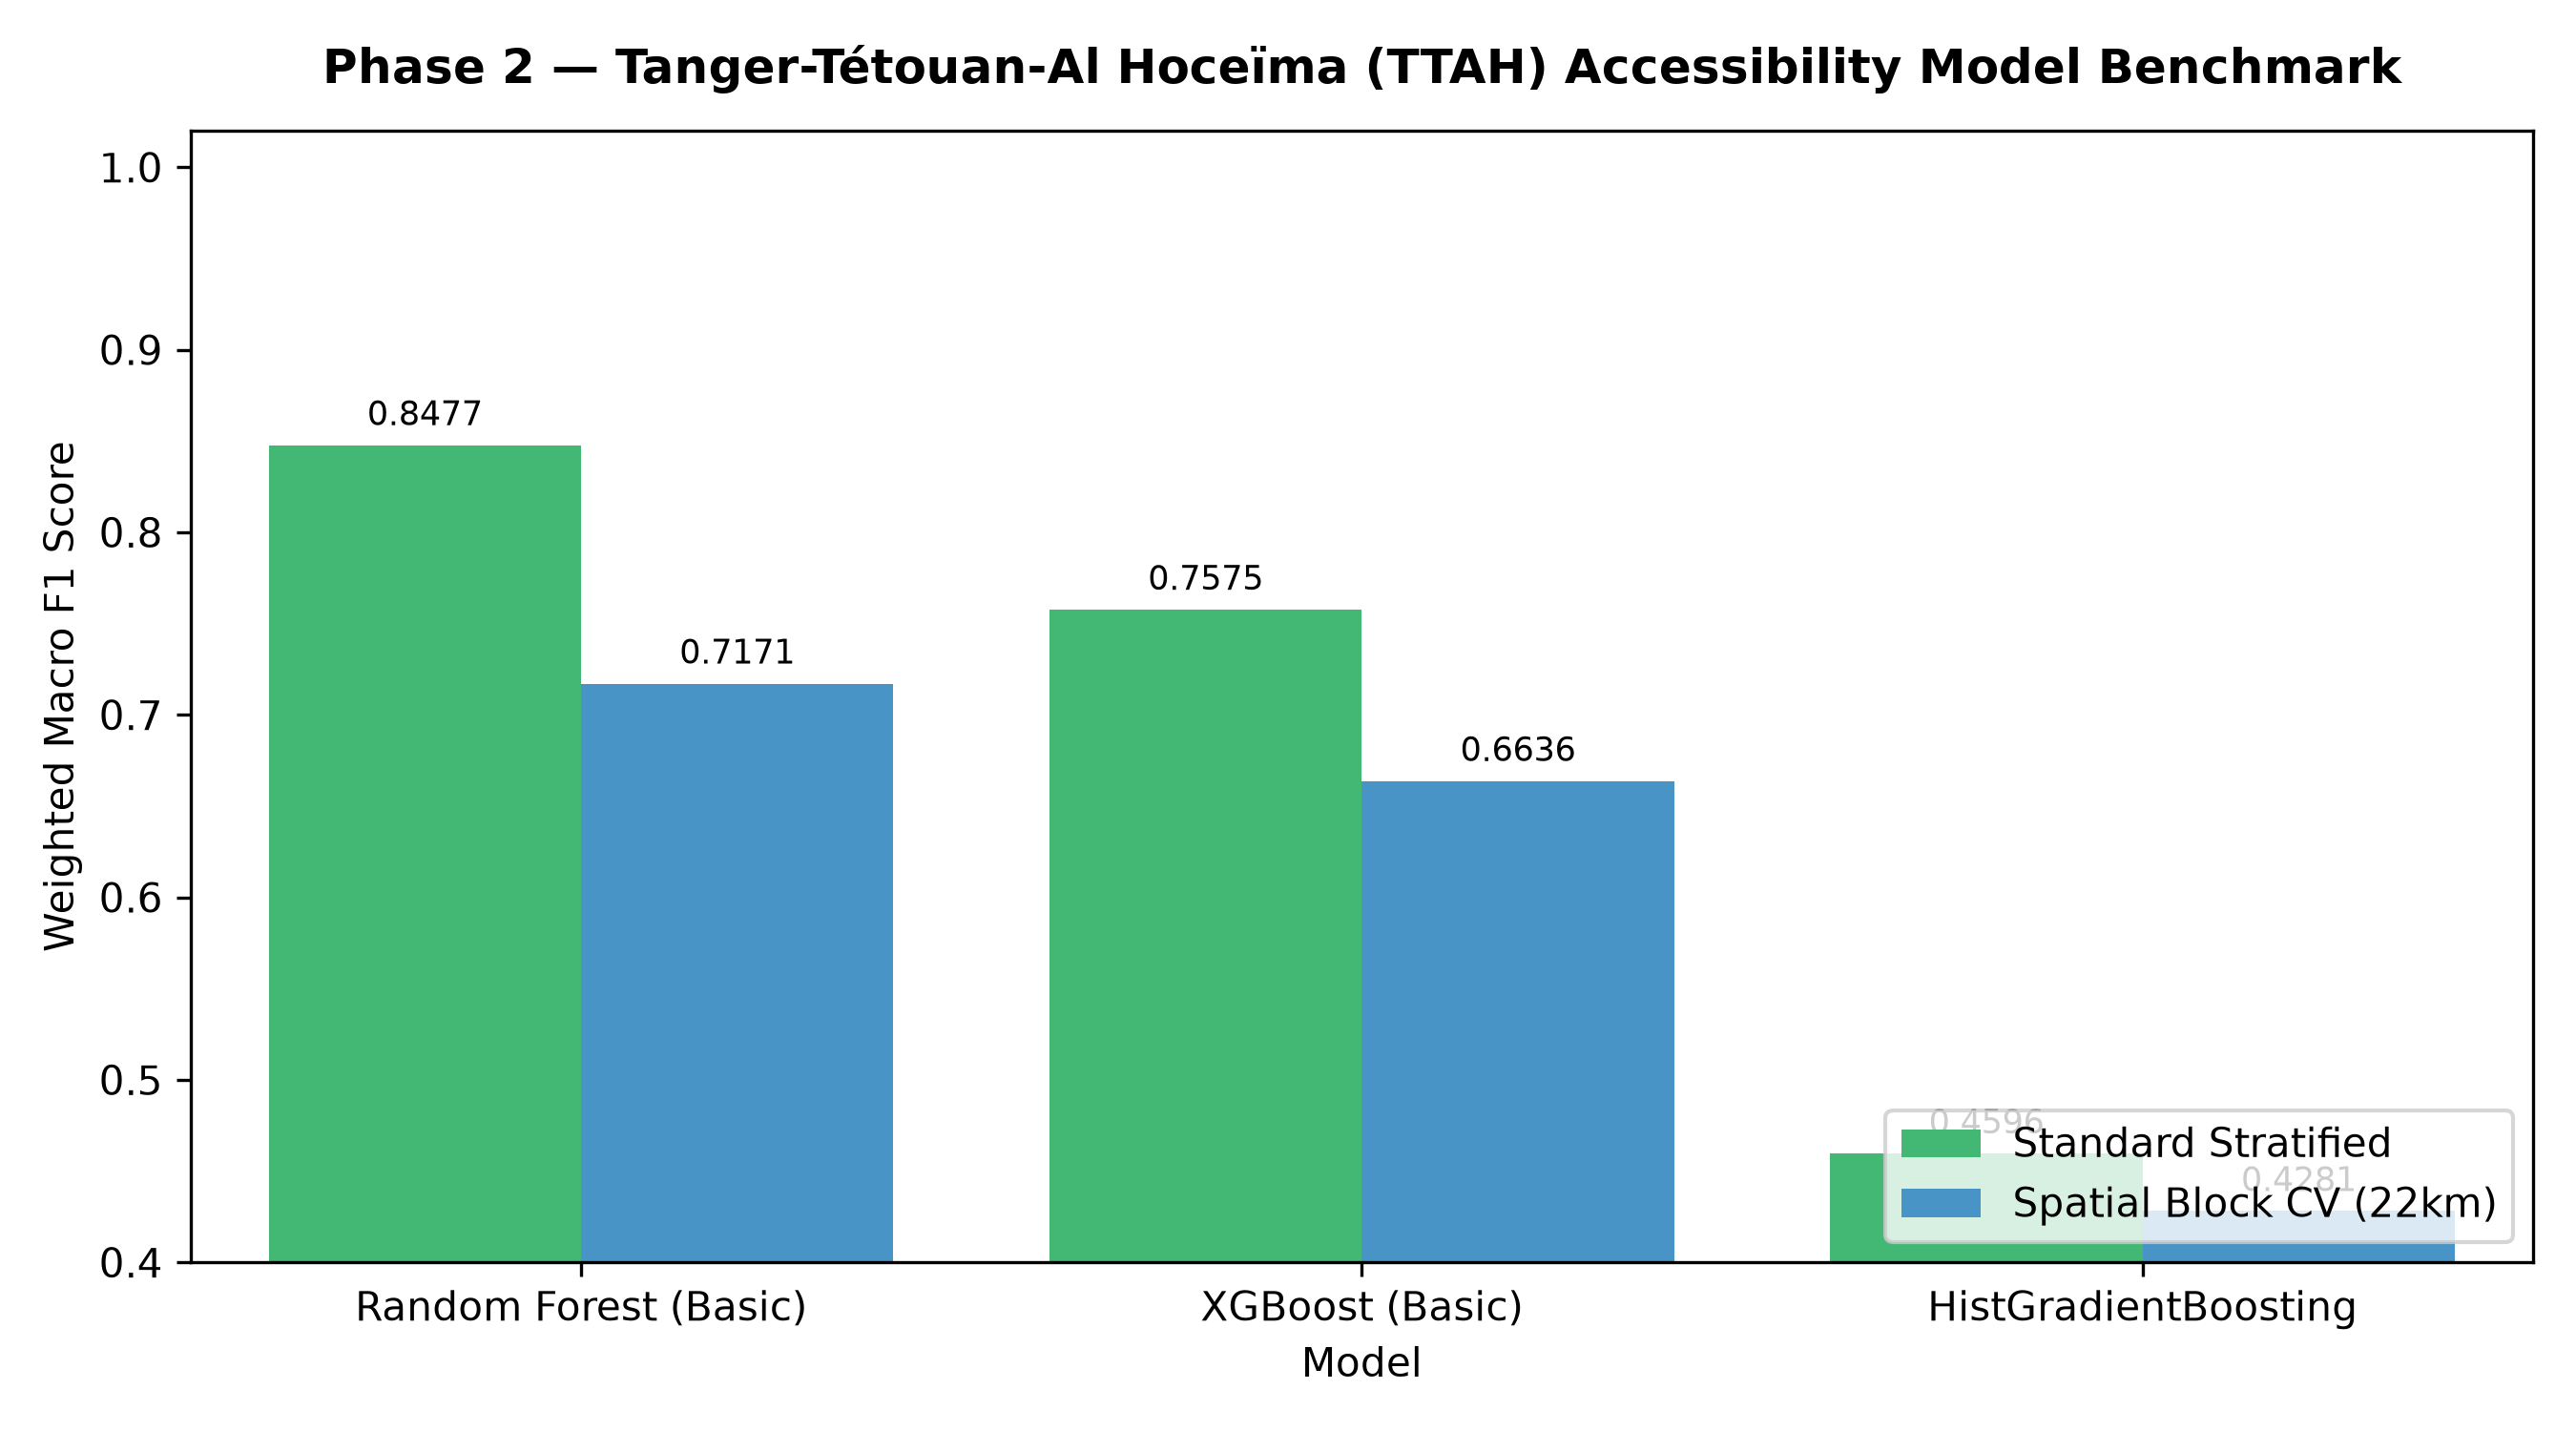
\includegraphics[width=\linewidth]{../figures/ttah_model_comparison.png}
    \caption{Comparaison des modèles prédictifs pour la région Tanger-Tétouan-Al Hoceïma (Standard CV F1 vs Spatial Block CV F1).}
    \label{fig:ttah_comp}
\end{figure}

\subsection{Justification Théorique et Empirique du Choix $K=5$}
La sélection du nombre de clusters $K$ pour le partitionnement non supervisé K-Means est étayée par la combinaison conjointe de trois métriques complémentaires (Figures \ref{fig:k_just} et \ref{fig:ttah_k_just}) :
\begin{enumerate}
    \item \textbf{Méthode Elbow (Inertie intra-classe)} : Pour BMK, l'inertie intra-classe chute fortement de $114,10$ ($K=2$) à $73,27$ ($K=3$) puis $53,87$ ($K=4$) avant de se stabiliser au coude d'inflexion à $K=5$ ($42,22$). Pour TTAH, l'inertie passe de $110,20$ ($K=2$) à $81,64$ ($K=3$) puis $61,65$ ($K=4$) avant d'atteindre un coude net à $K=5$ ($48,71$). Augmenter $K > 5$ n'apporte qu'une réduction marginale de variance.
    \item \textbf{Score Silhouette ($S_{\text{sil}}$)} : Pour BMK, le score silhouette atteint $0,3642$ ($K=3$) et $0,3619$ ($K=4$), puis se stabilise à $0,3515$ à $K=5$. Pour TTAH, sur le plan strictement mathématique, $K=6$ atteint le score silhouette maximal ($0,3371$ vs. $0,3315$ pour $K=5$).
    \item \textbf{Index de Davies-Bouldin ($DB$)} : Pour BMK, l'index $DB$ atteint son minimum local à $K=5$ (\textbf{$0,9052$}). Pour TTAH, $DB$ poursuit sa baisse à $K=6$ (\textbf{$0,9120$} vs. $0,9365$ à $K=5$). Sur TTAH, bien que $K=6$ constitue l'optimum mathématique pur, le choix de $K=5$ est maintenu pour des motifs d'harmonisation inter-régionale des 5 profils de gestion et pour éviter la sur-fragmentation d'échantillon ($N=51$).
\end{enumerate}

\begin{figure*}[t]
    \centering
    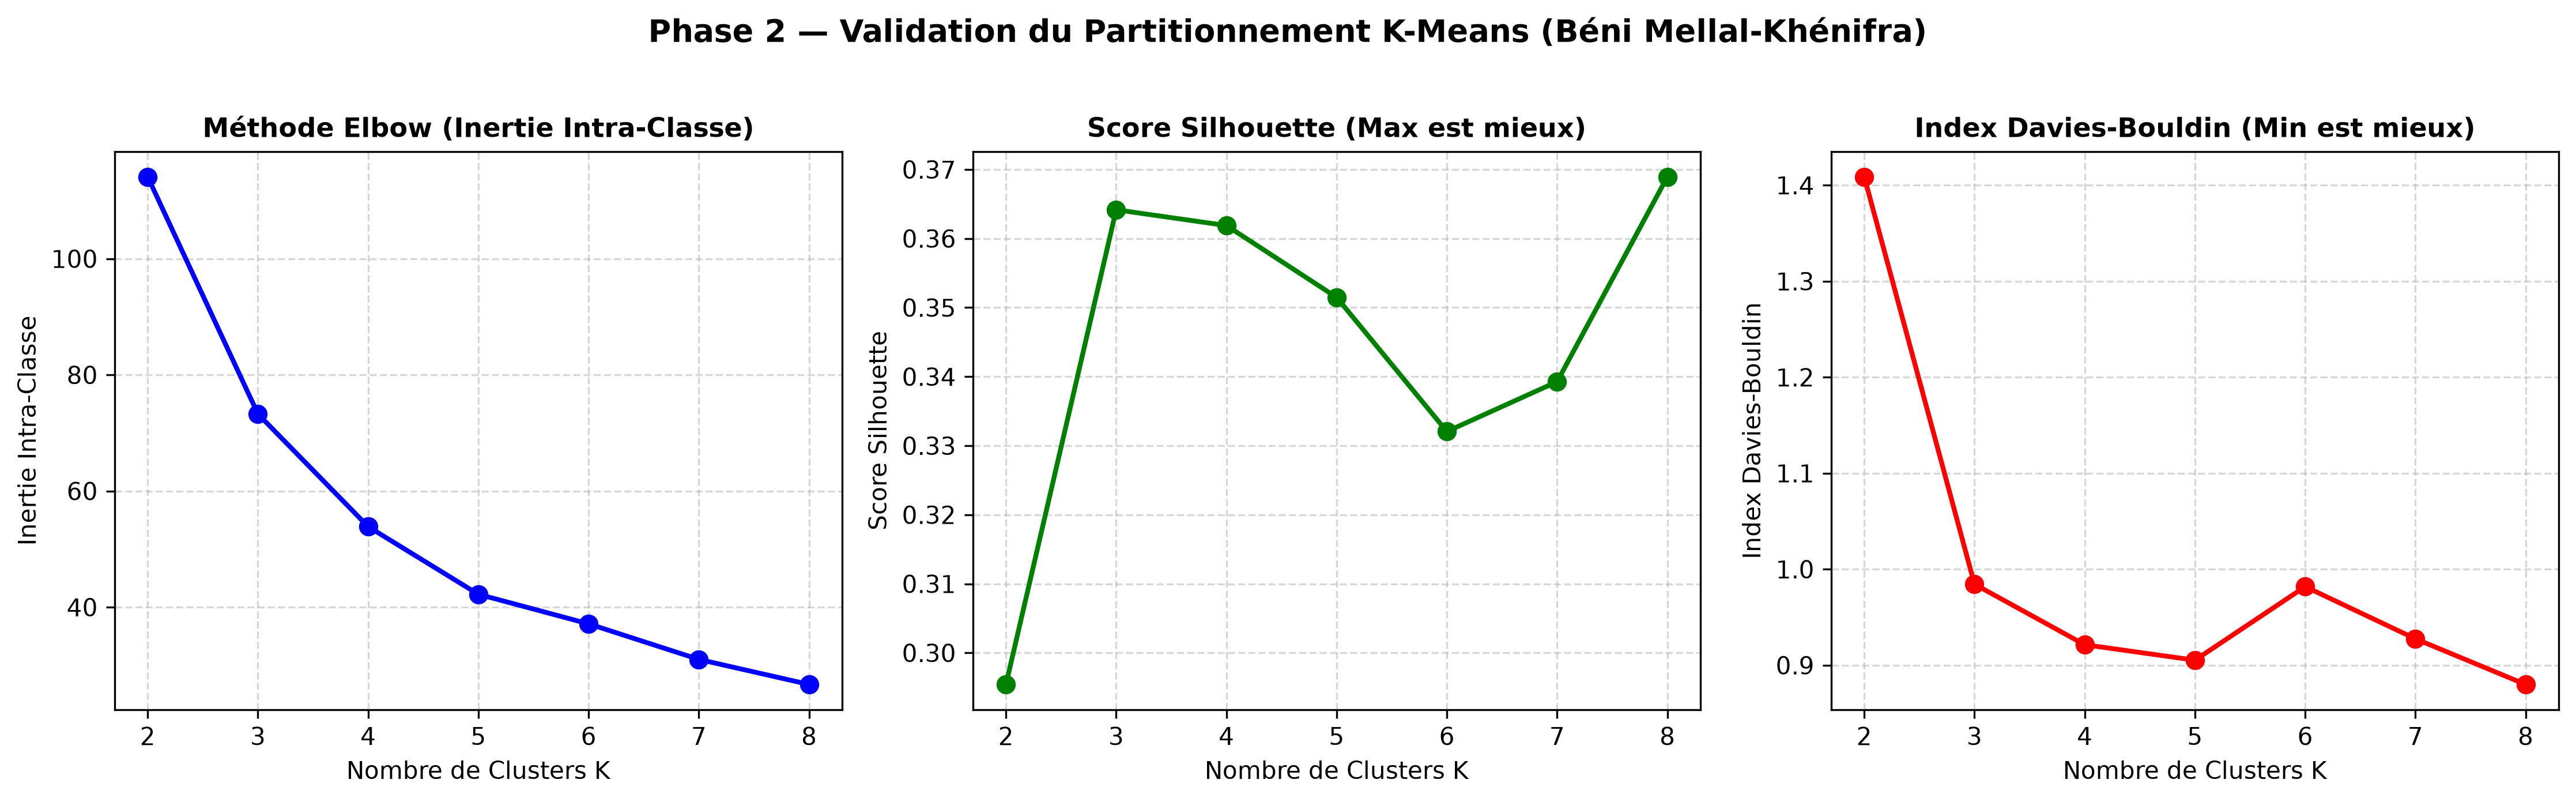
\includegraphics[width=0.92\linewidth]{../figures/kmeans_k_justification.png}
    \caption{Analyse de validation du partitionnement K-Means ($N=55$ géosites de Béni Mellal-Khénifra). De gauche à droite : courbe de l'inertie intra-classe (Elbow), score Silhouette (max est mieux), et index de Davies-Bouldin (min est mieux), justifiant la sélection optimale de $K=5$ clusters.}
    \label{fig:k_just}
\end{figure*}

\begin{figure*}[t]
    \centering
    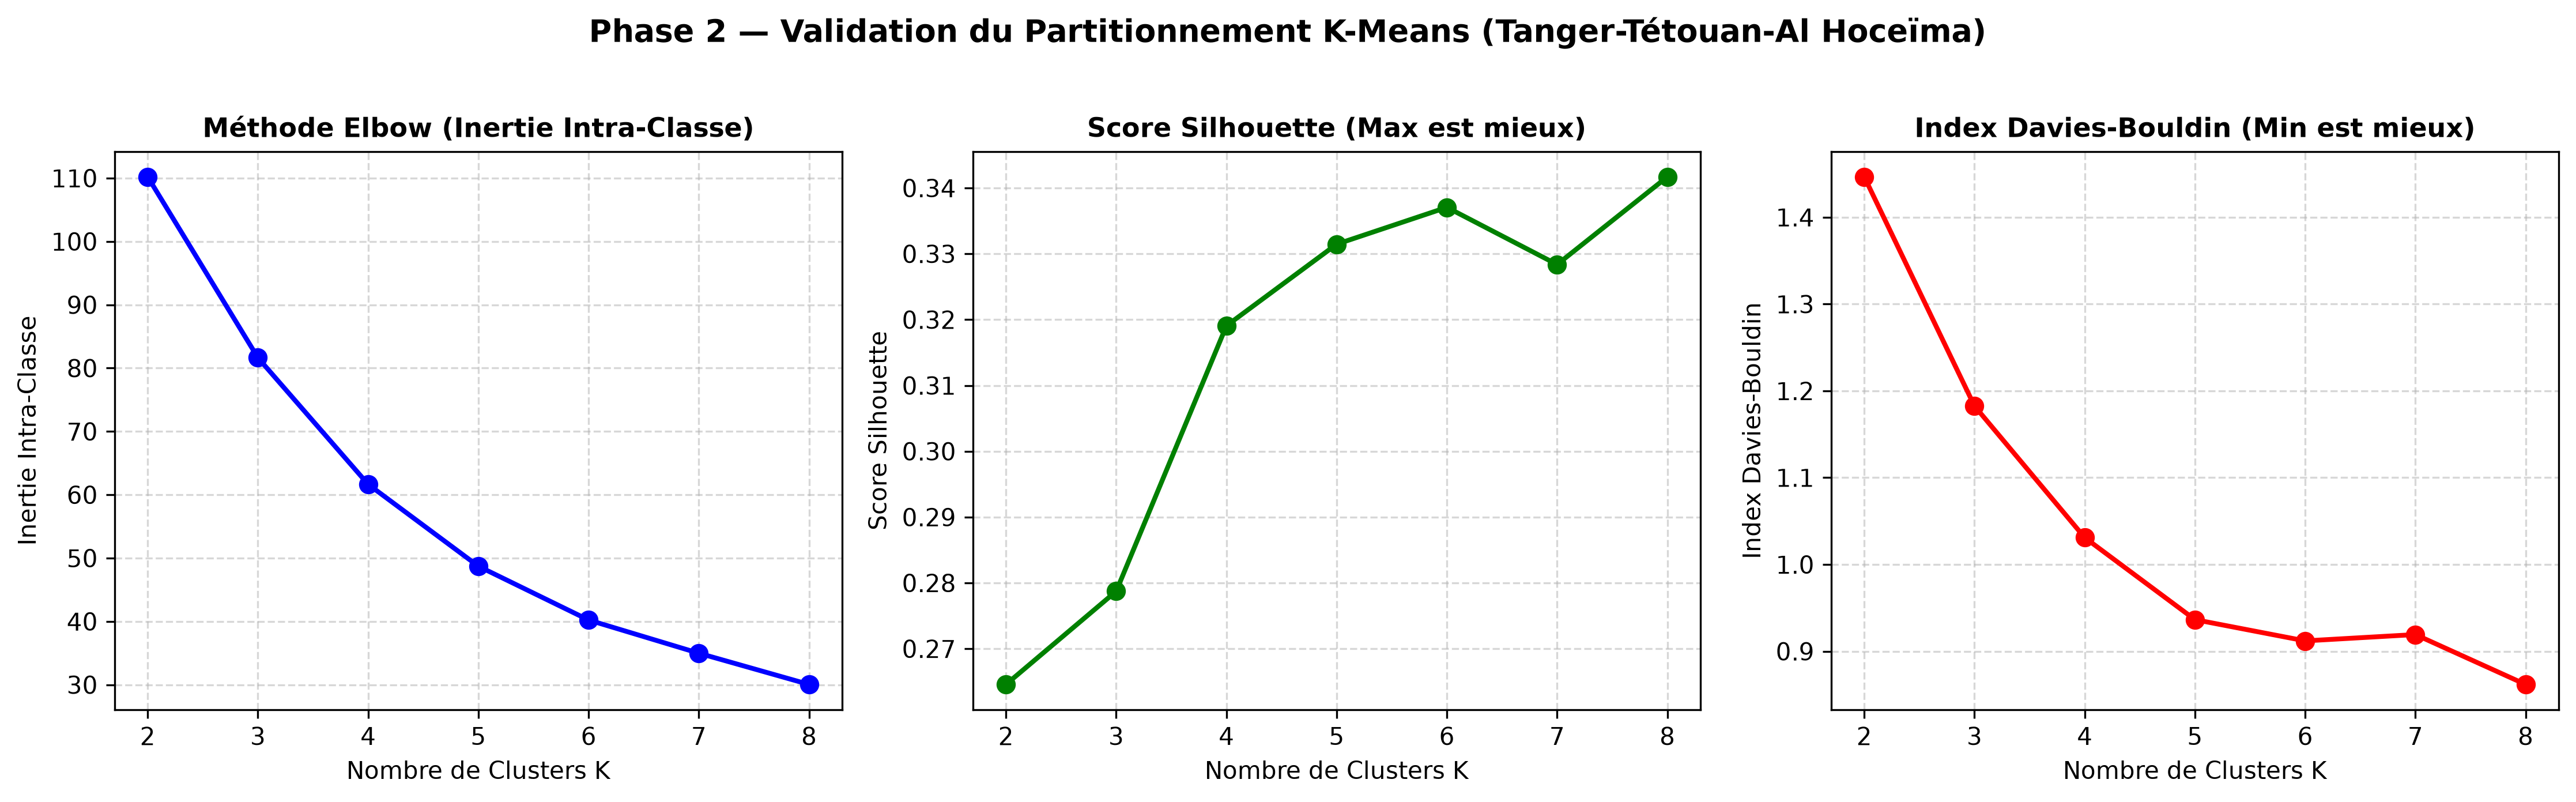
\includegraphics[width=0.92\linewidth]{../figures/ttah_kmeans_k_justification.png}
    \caption{Analyse de validation du partitionnement K-Means ($N=51$ géosites de Tanger-Tétouan-Al Hoceïma), confirmant le choix de $K=5$ clusters pour la caractérisation des profils de gestion.}
    \label{fig:ttah_k_just}
\end{figure*}

Le choix de $K=5$ offre ainsi le compromis mathématique et métier optimal, permettant de caractériser les cinq profils opérationnels de gestion suivants :
\begin{enumerate}
    \item \textbf{Préservation Absolue (Sanctuaire)} : géosites à très haute valeur scientifique mais d'accès extrêmement difficile et forte vulnérabilité.
    \item \textbf{Préservation Passive (Accès difficile)} : sites isolés nécessitant un contrôle d'accès.
    \item \textbf{Conservation Active (Sensibilité physique)} : sites accessibles mais soumis à une érosion physique marquée.
    \item \textbf{Promotion Éducative (Grand Public)} : géosites très accessibles ($S_{\text{access}} \ge 0.50$), faible vulnérabilité, adaptés aux visites scolaires.
    \item \textbf{Promotion Géotouristique Locale} : sites accessibles en vallée ou littoral à haut potentiel de développement éco-touristique.
\end{enumerate}

Les Figures \ref{fig:bmk_3d} et \ref{fig:ttah_3d} présentent la répartition spatiale 3D des clusters dans l'espace des attributs (Valeur Scientifique, Vulnérabilité, Score Flou d'Accessibilité).

\begin{figure}[htbp]
    \centering
    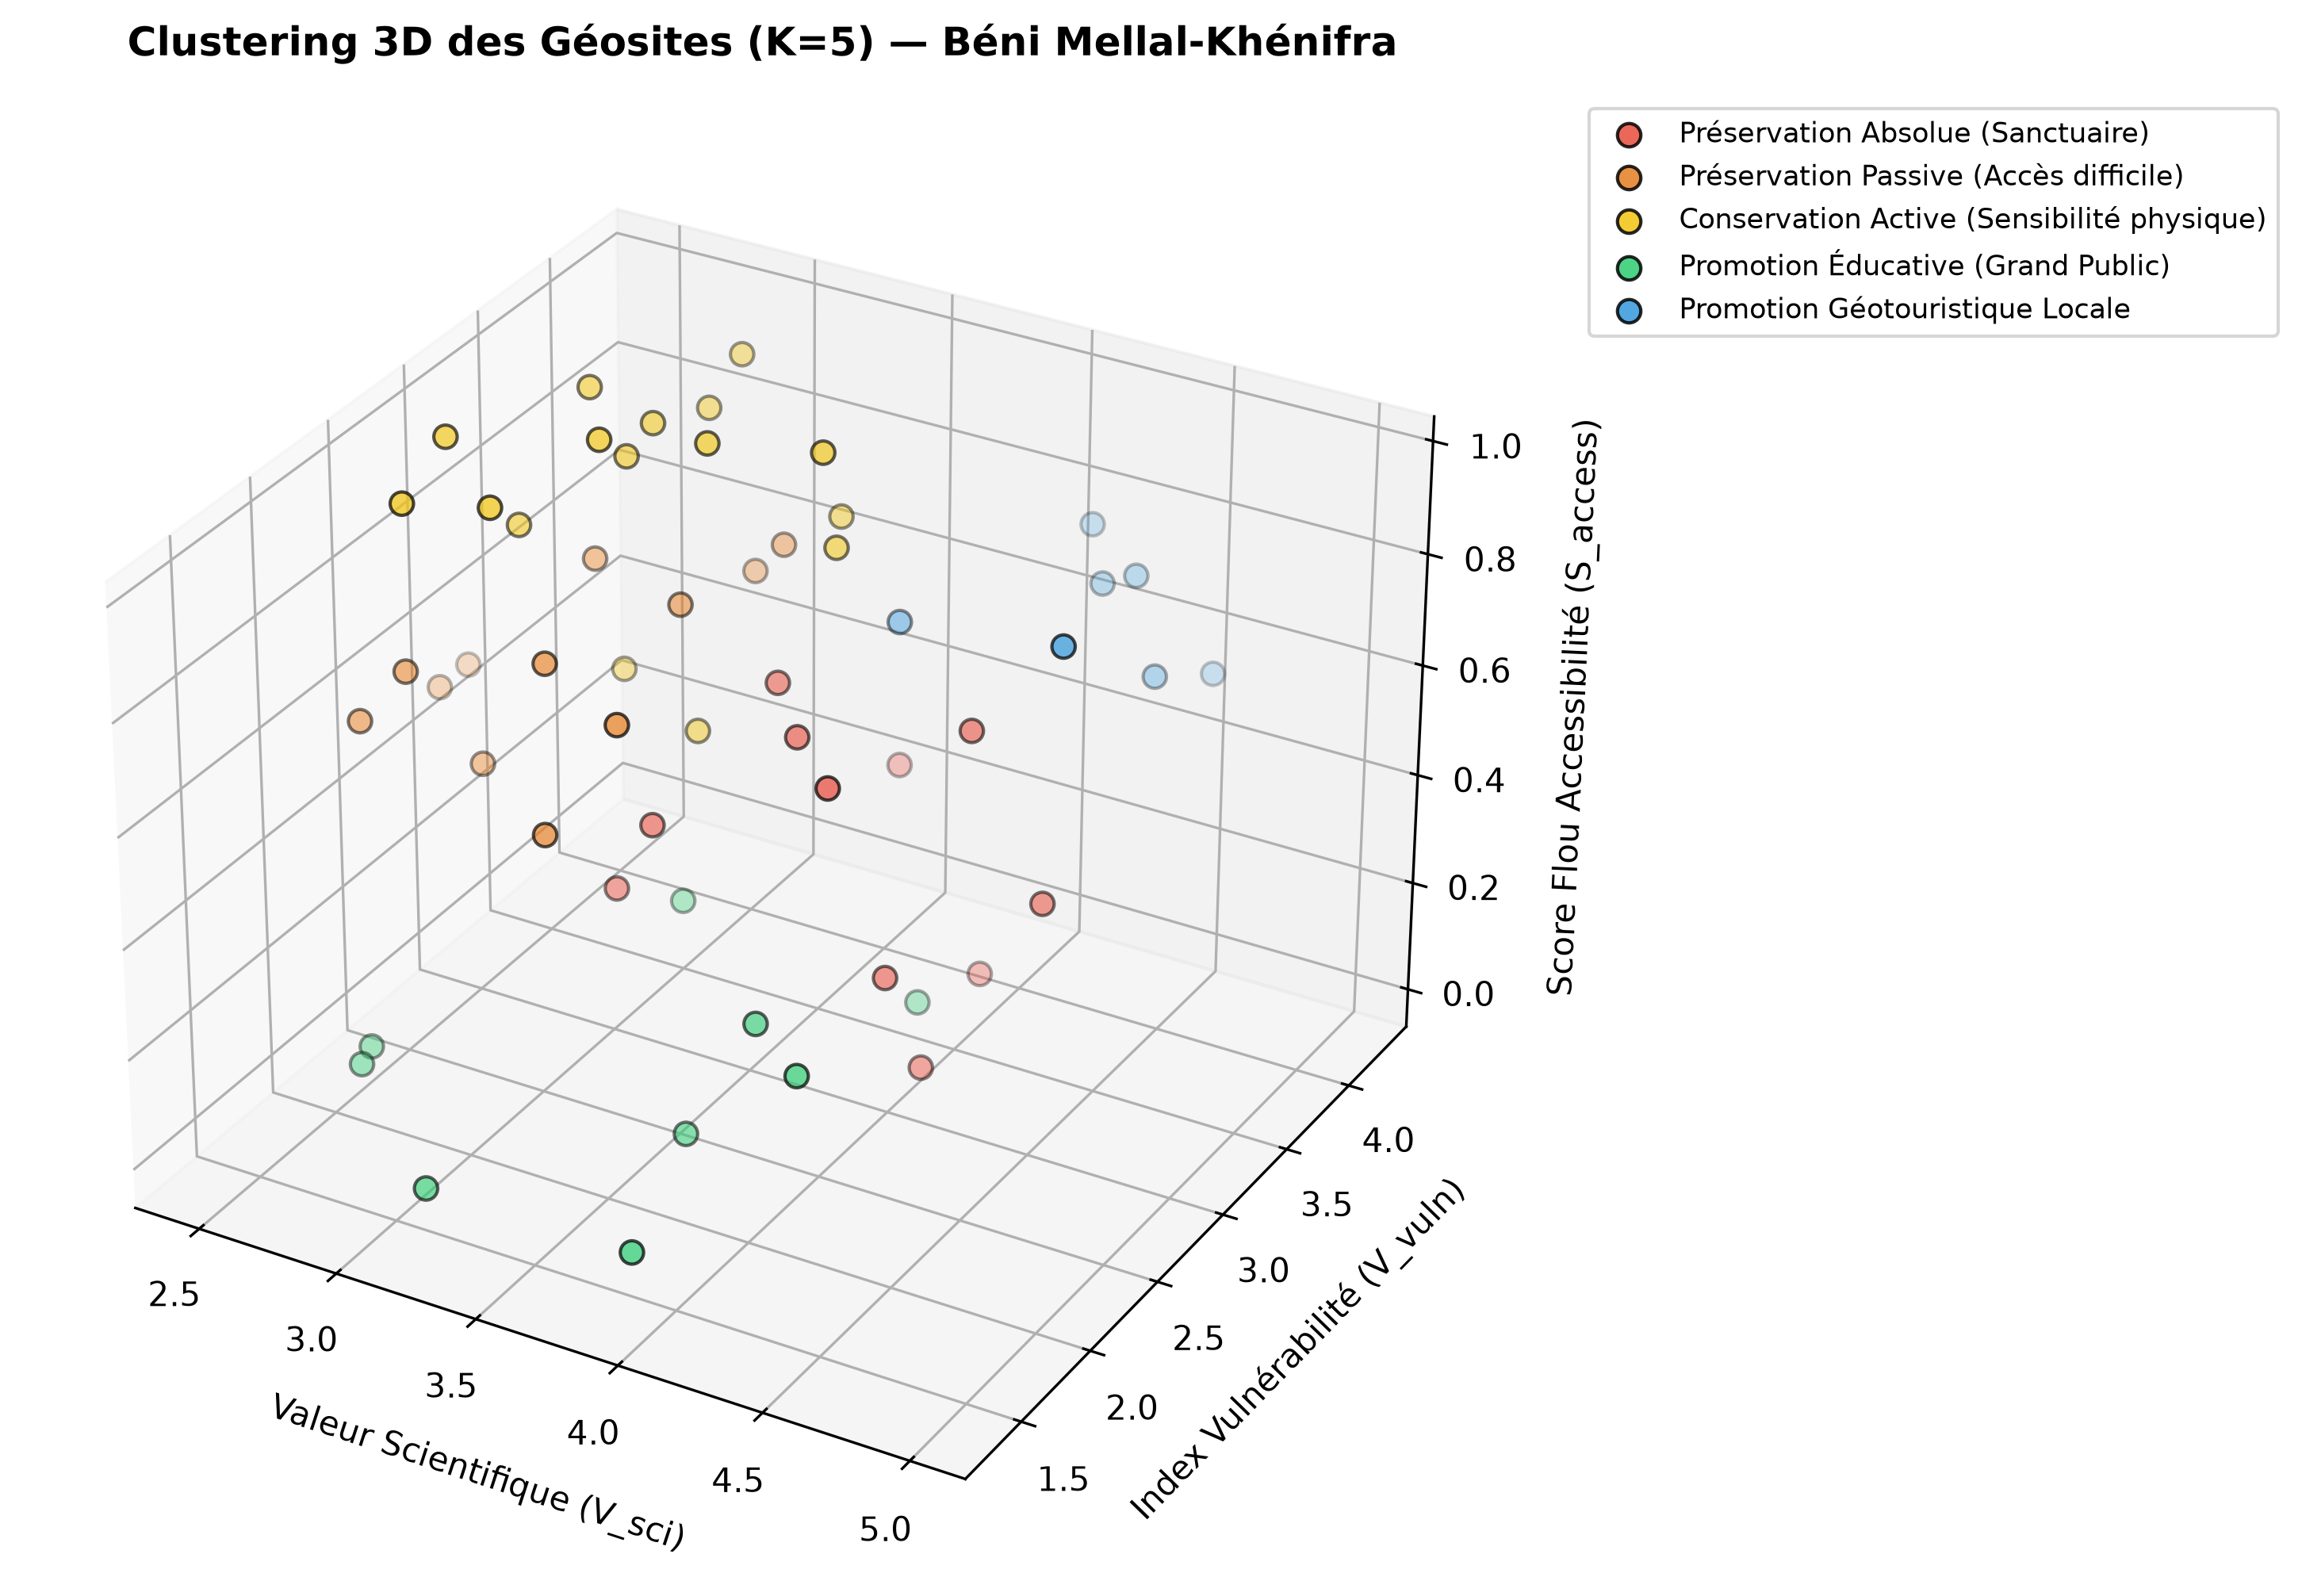
\includegraphics[width=\linewidth]{../figures/geosites_3d_clustering.png}
    \caption{Visualisation 3D du clustering K-Means des géosites pour Béni Mellal-Khénifra.}
    \label{fig:bmk_3d}
\end{figure}

\begin{figure}[htbp]
    \centering
    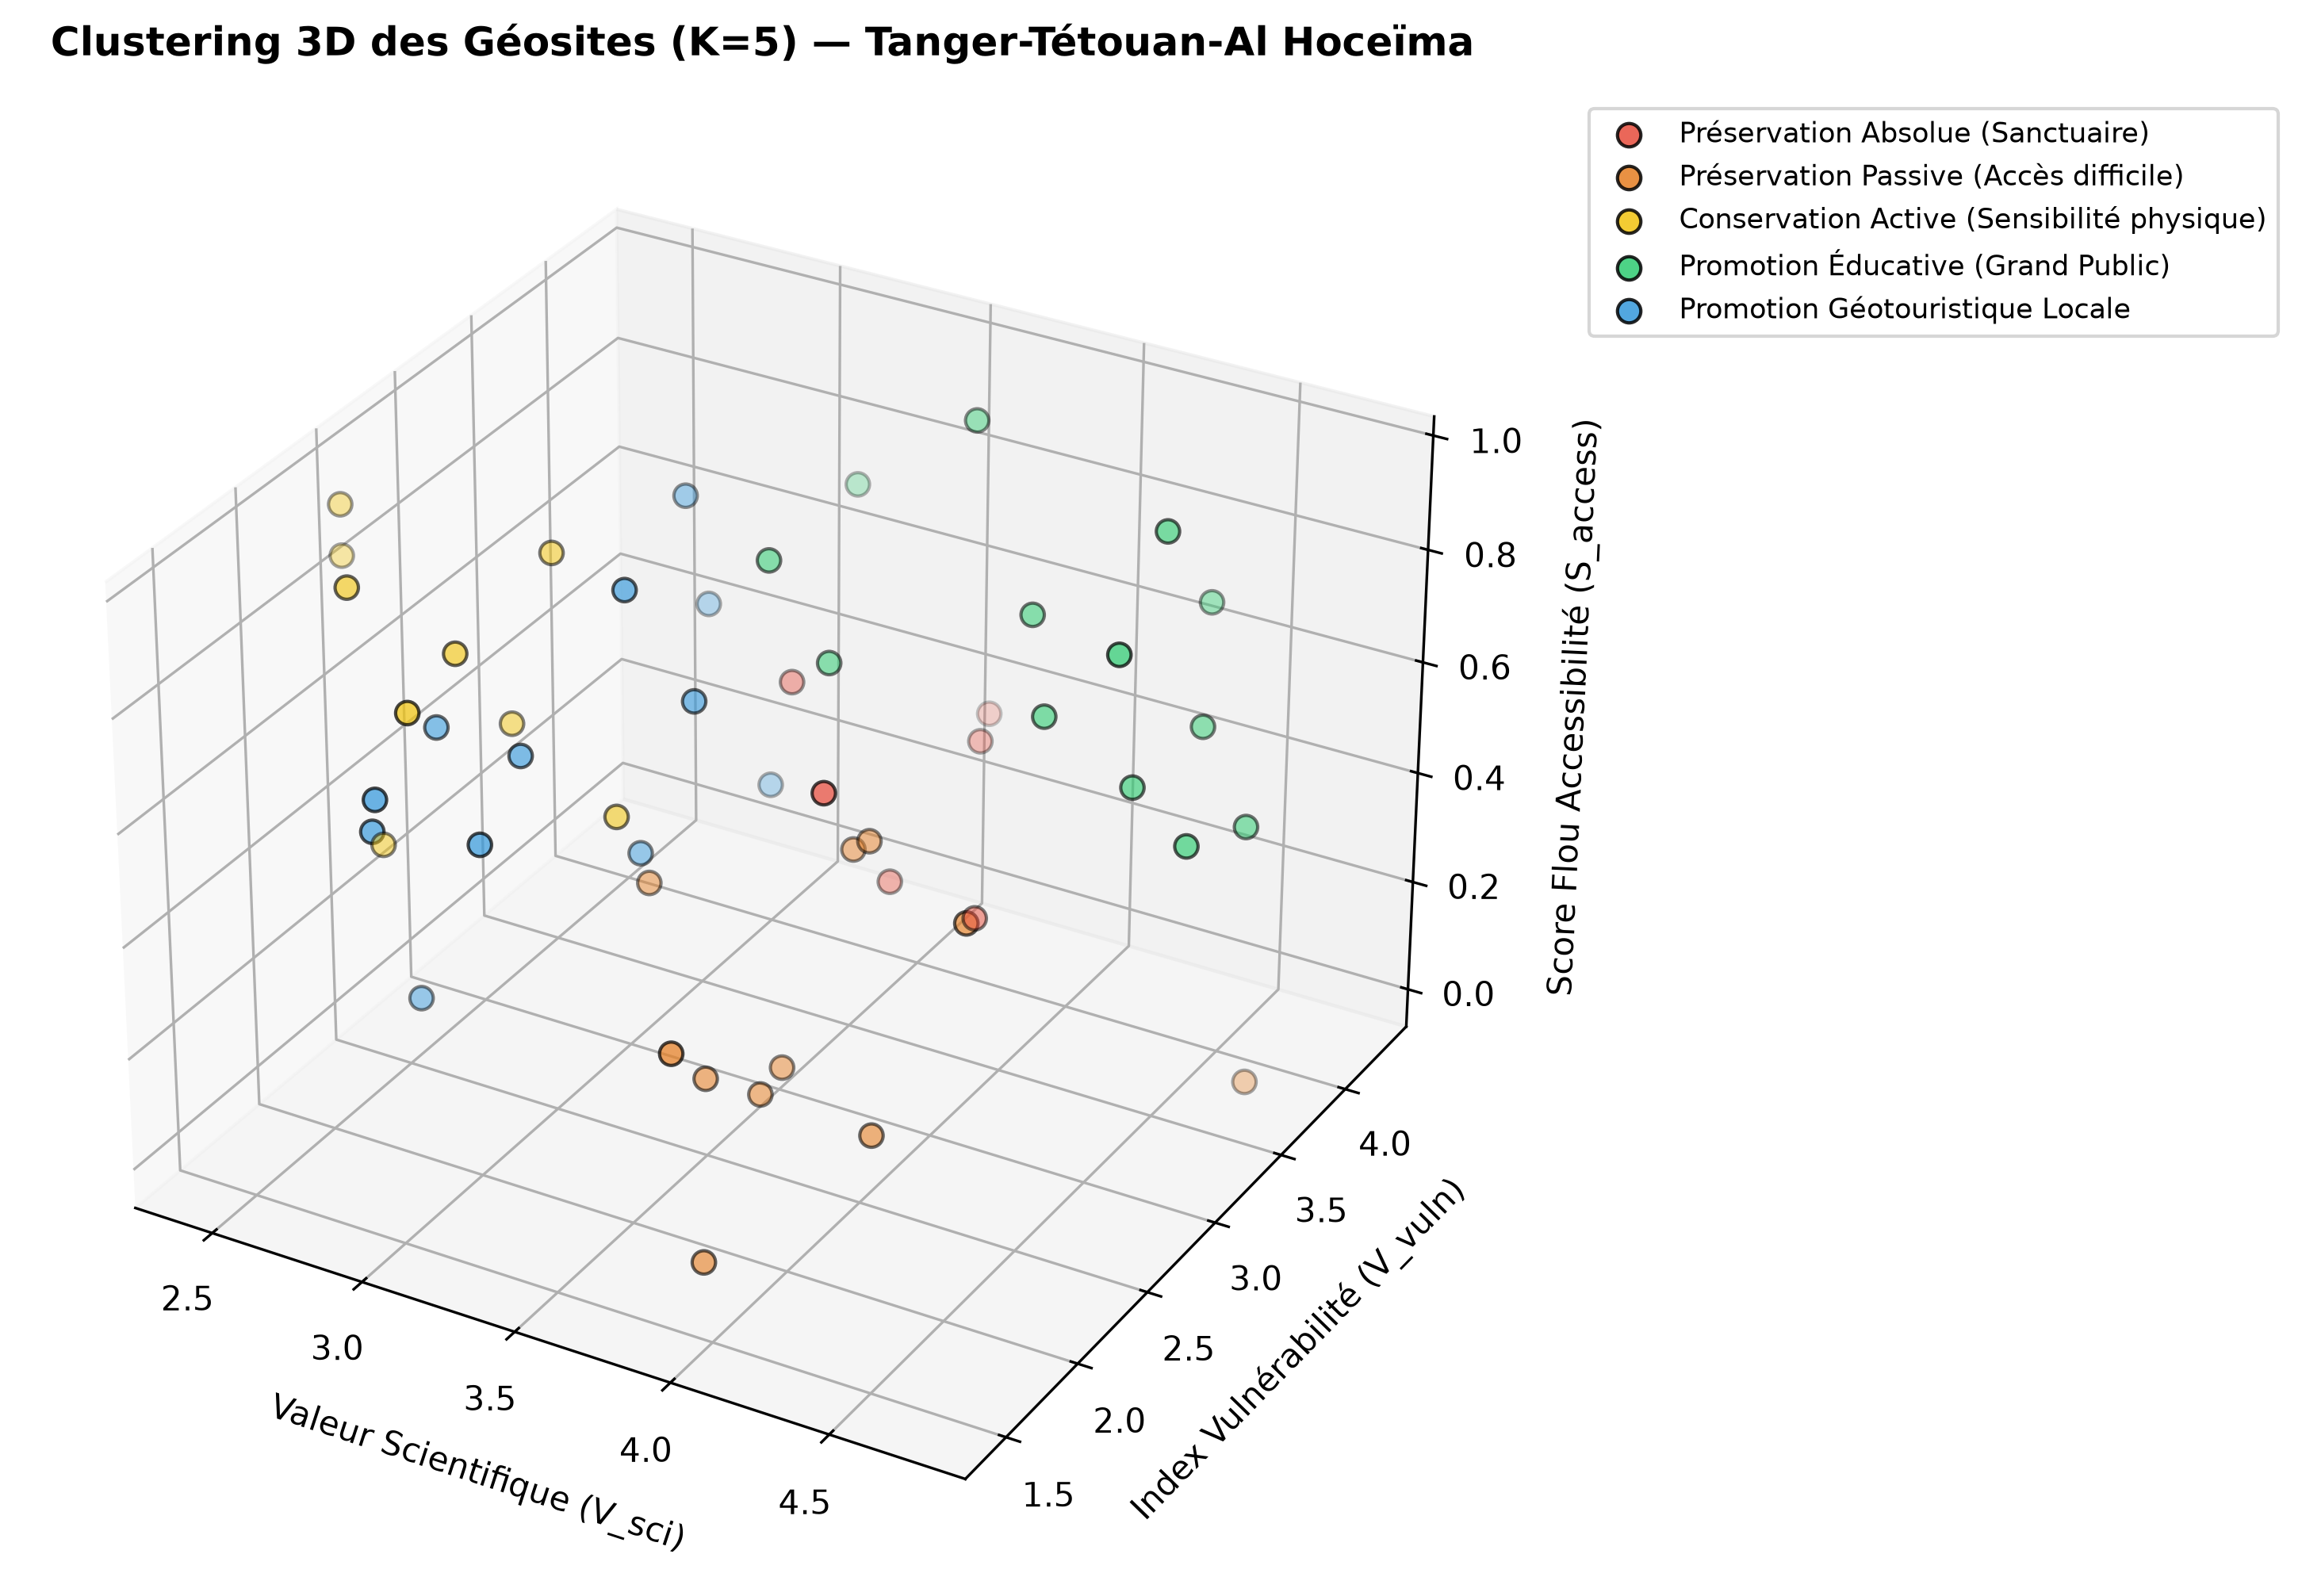
\includegraphics[width=\linewidth]{../figures/ttah_geosites_3d_clustering.png}
    \caption{Visualisation 3D du clustering K-Means des géosites pour Tanger-Tétouan-Al Hoceïma.}
    \label{fig:ttah_3d}
\end{figure}

Les Figures \ref{fig:bmk_spat_clust} et \ref{fig:ttah_spat_clust} illustrent la répartition géographique des profils de gestion strictement ancrés à l'intérieur des limites administratives régionales.

\begin{figure}[htbp]
    \centering
    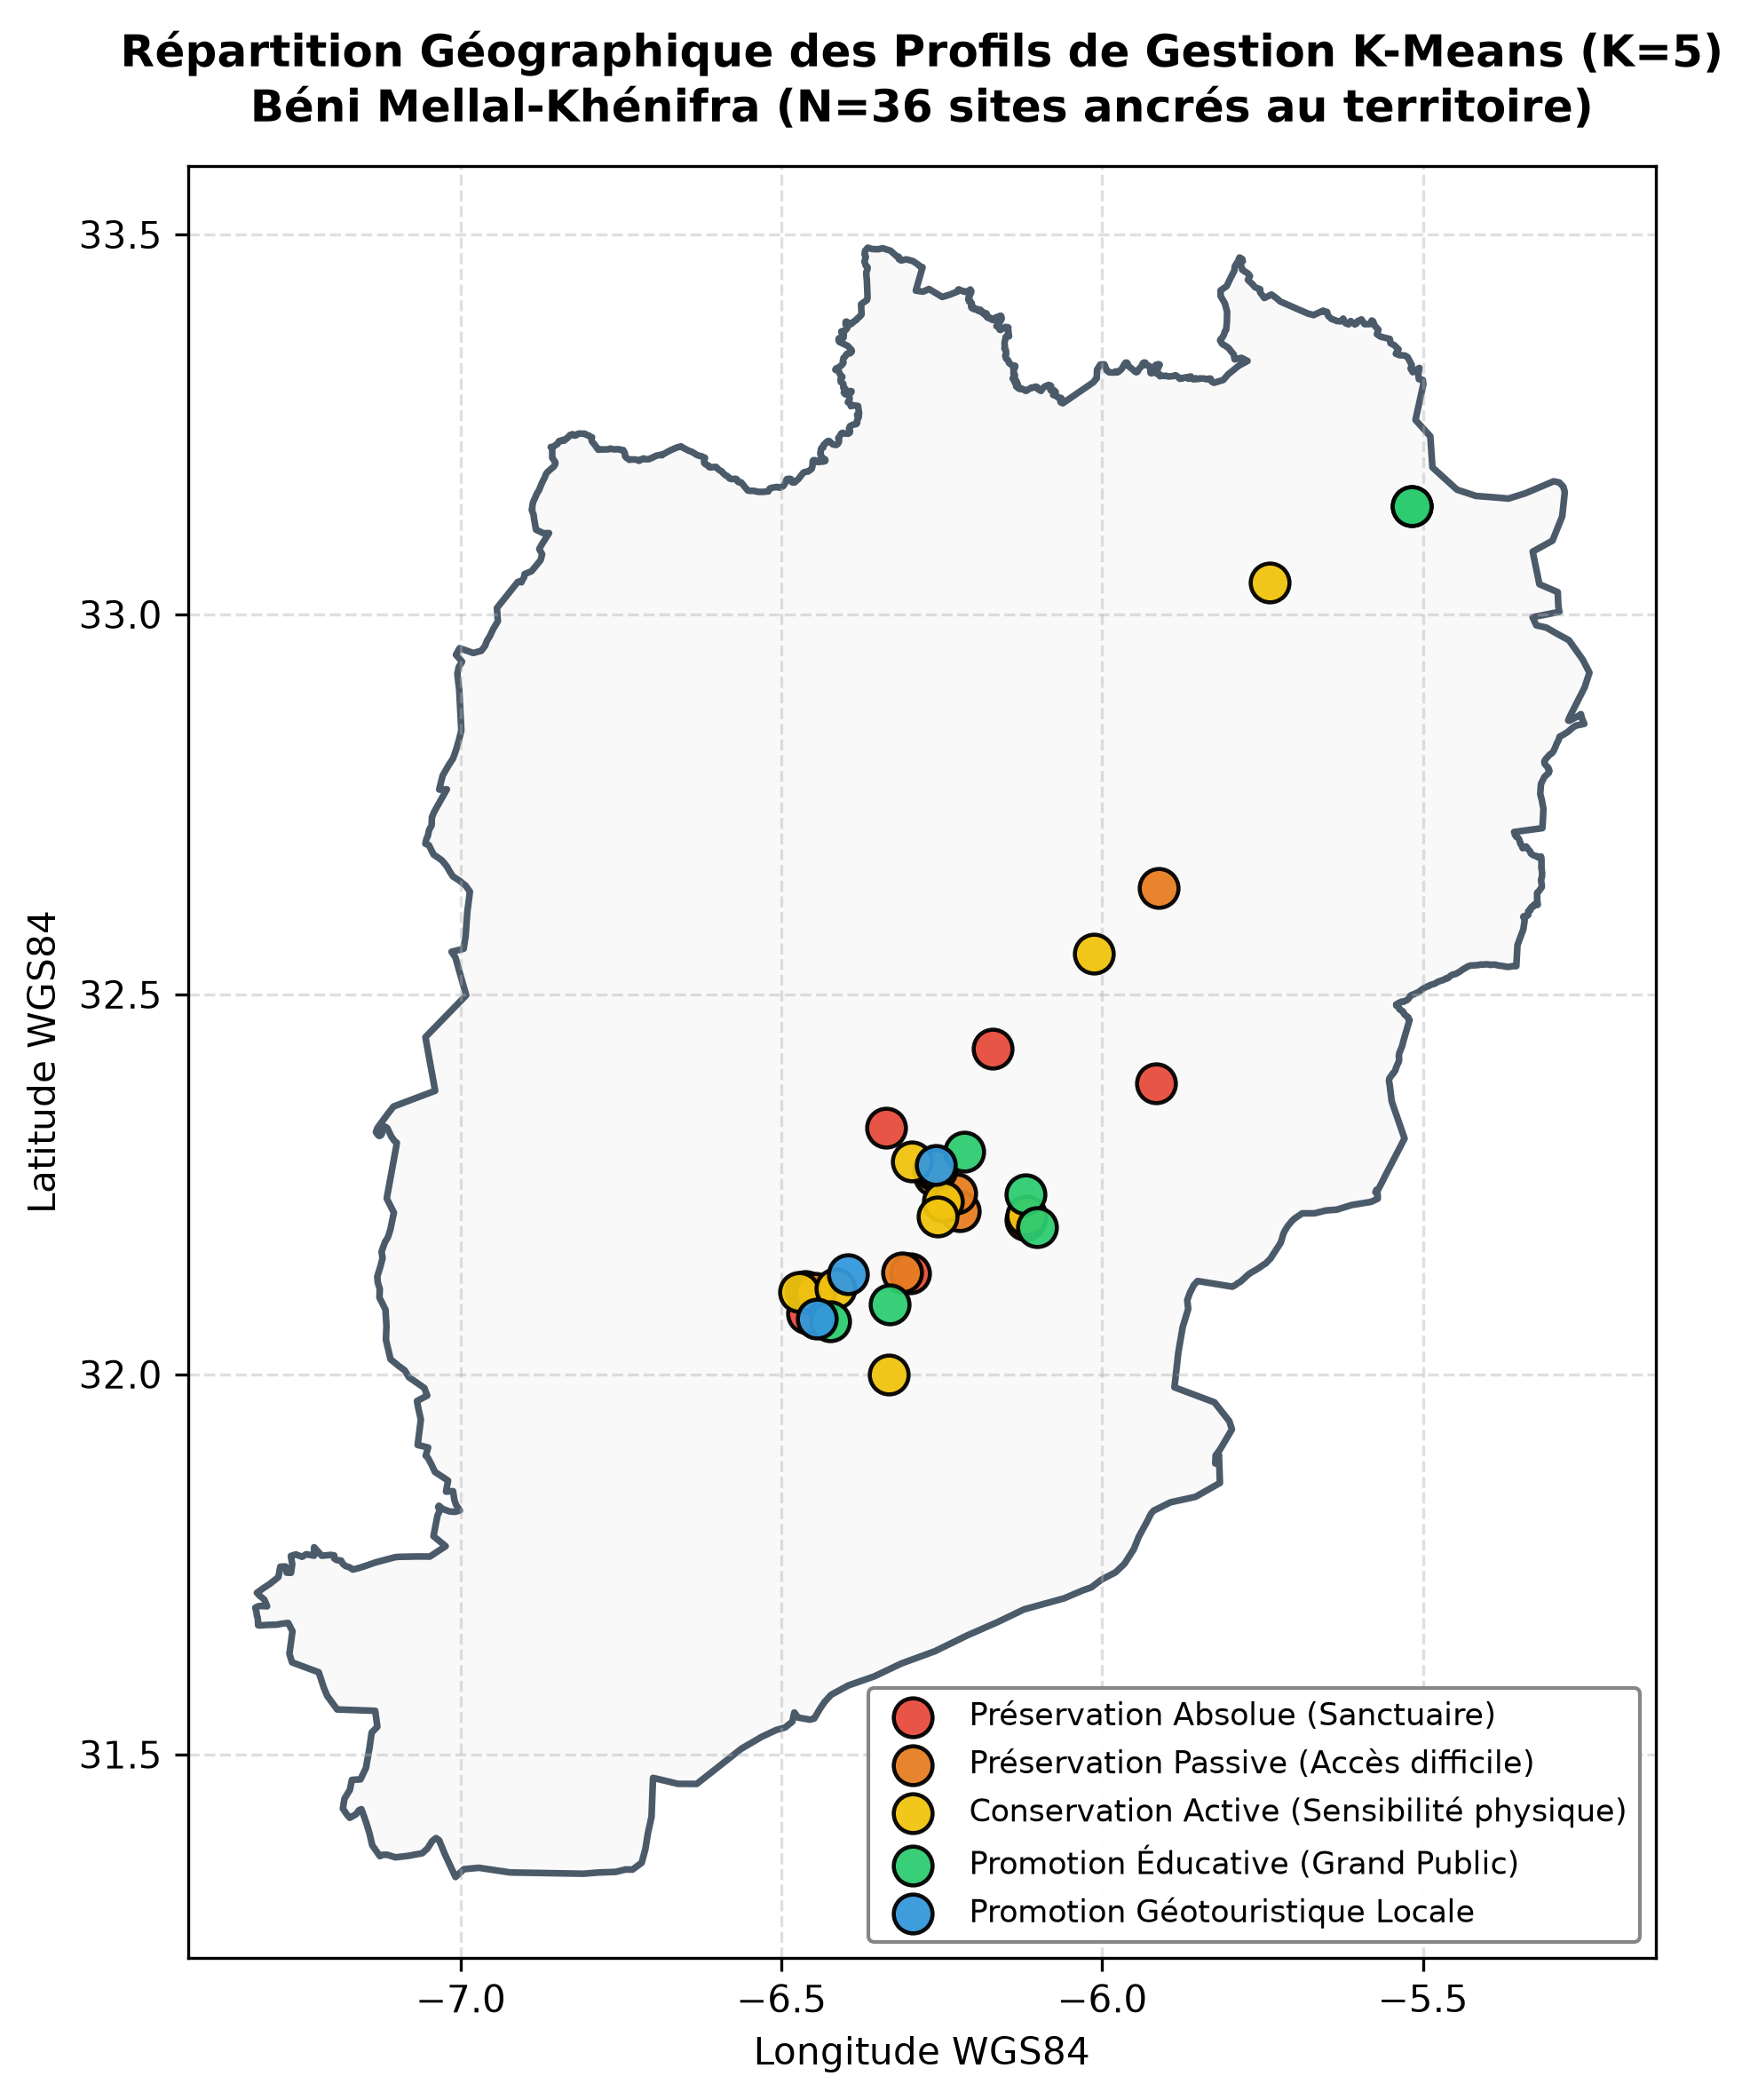
\includegraphics[width=\linewidth]{../figures/geosites_spatial_clusters.png}
    \caption{Répartition géographique des profils de gestion K-Means pour la région Béni Mellal-Khénifra ($N=36$ géosites strictement situés à l'intérieur du territoire provincial).}
    \label{fig:bmk_spat_clust}
\end{figure}

\begin{figure}[htbp]
    \centering
    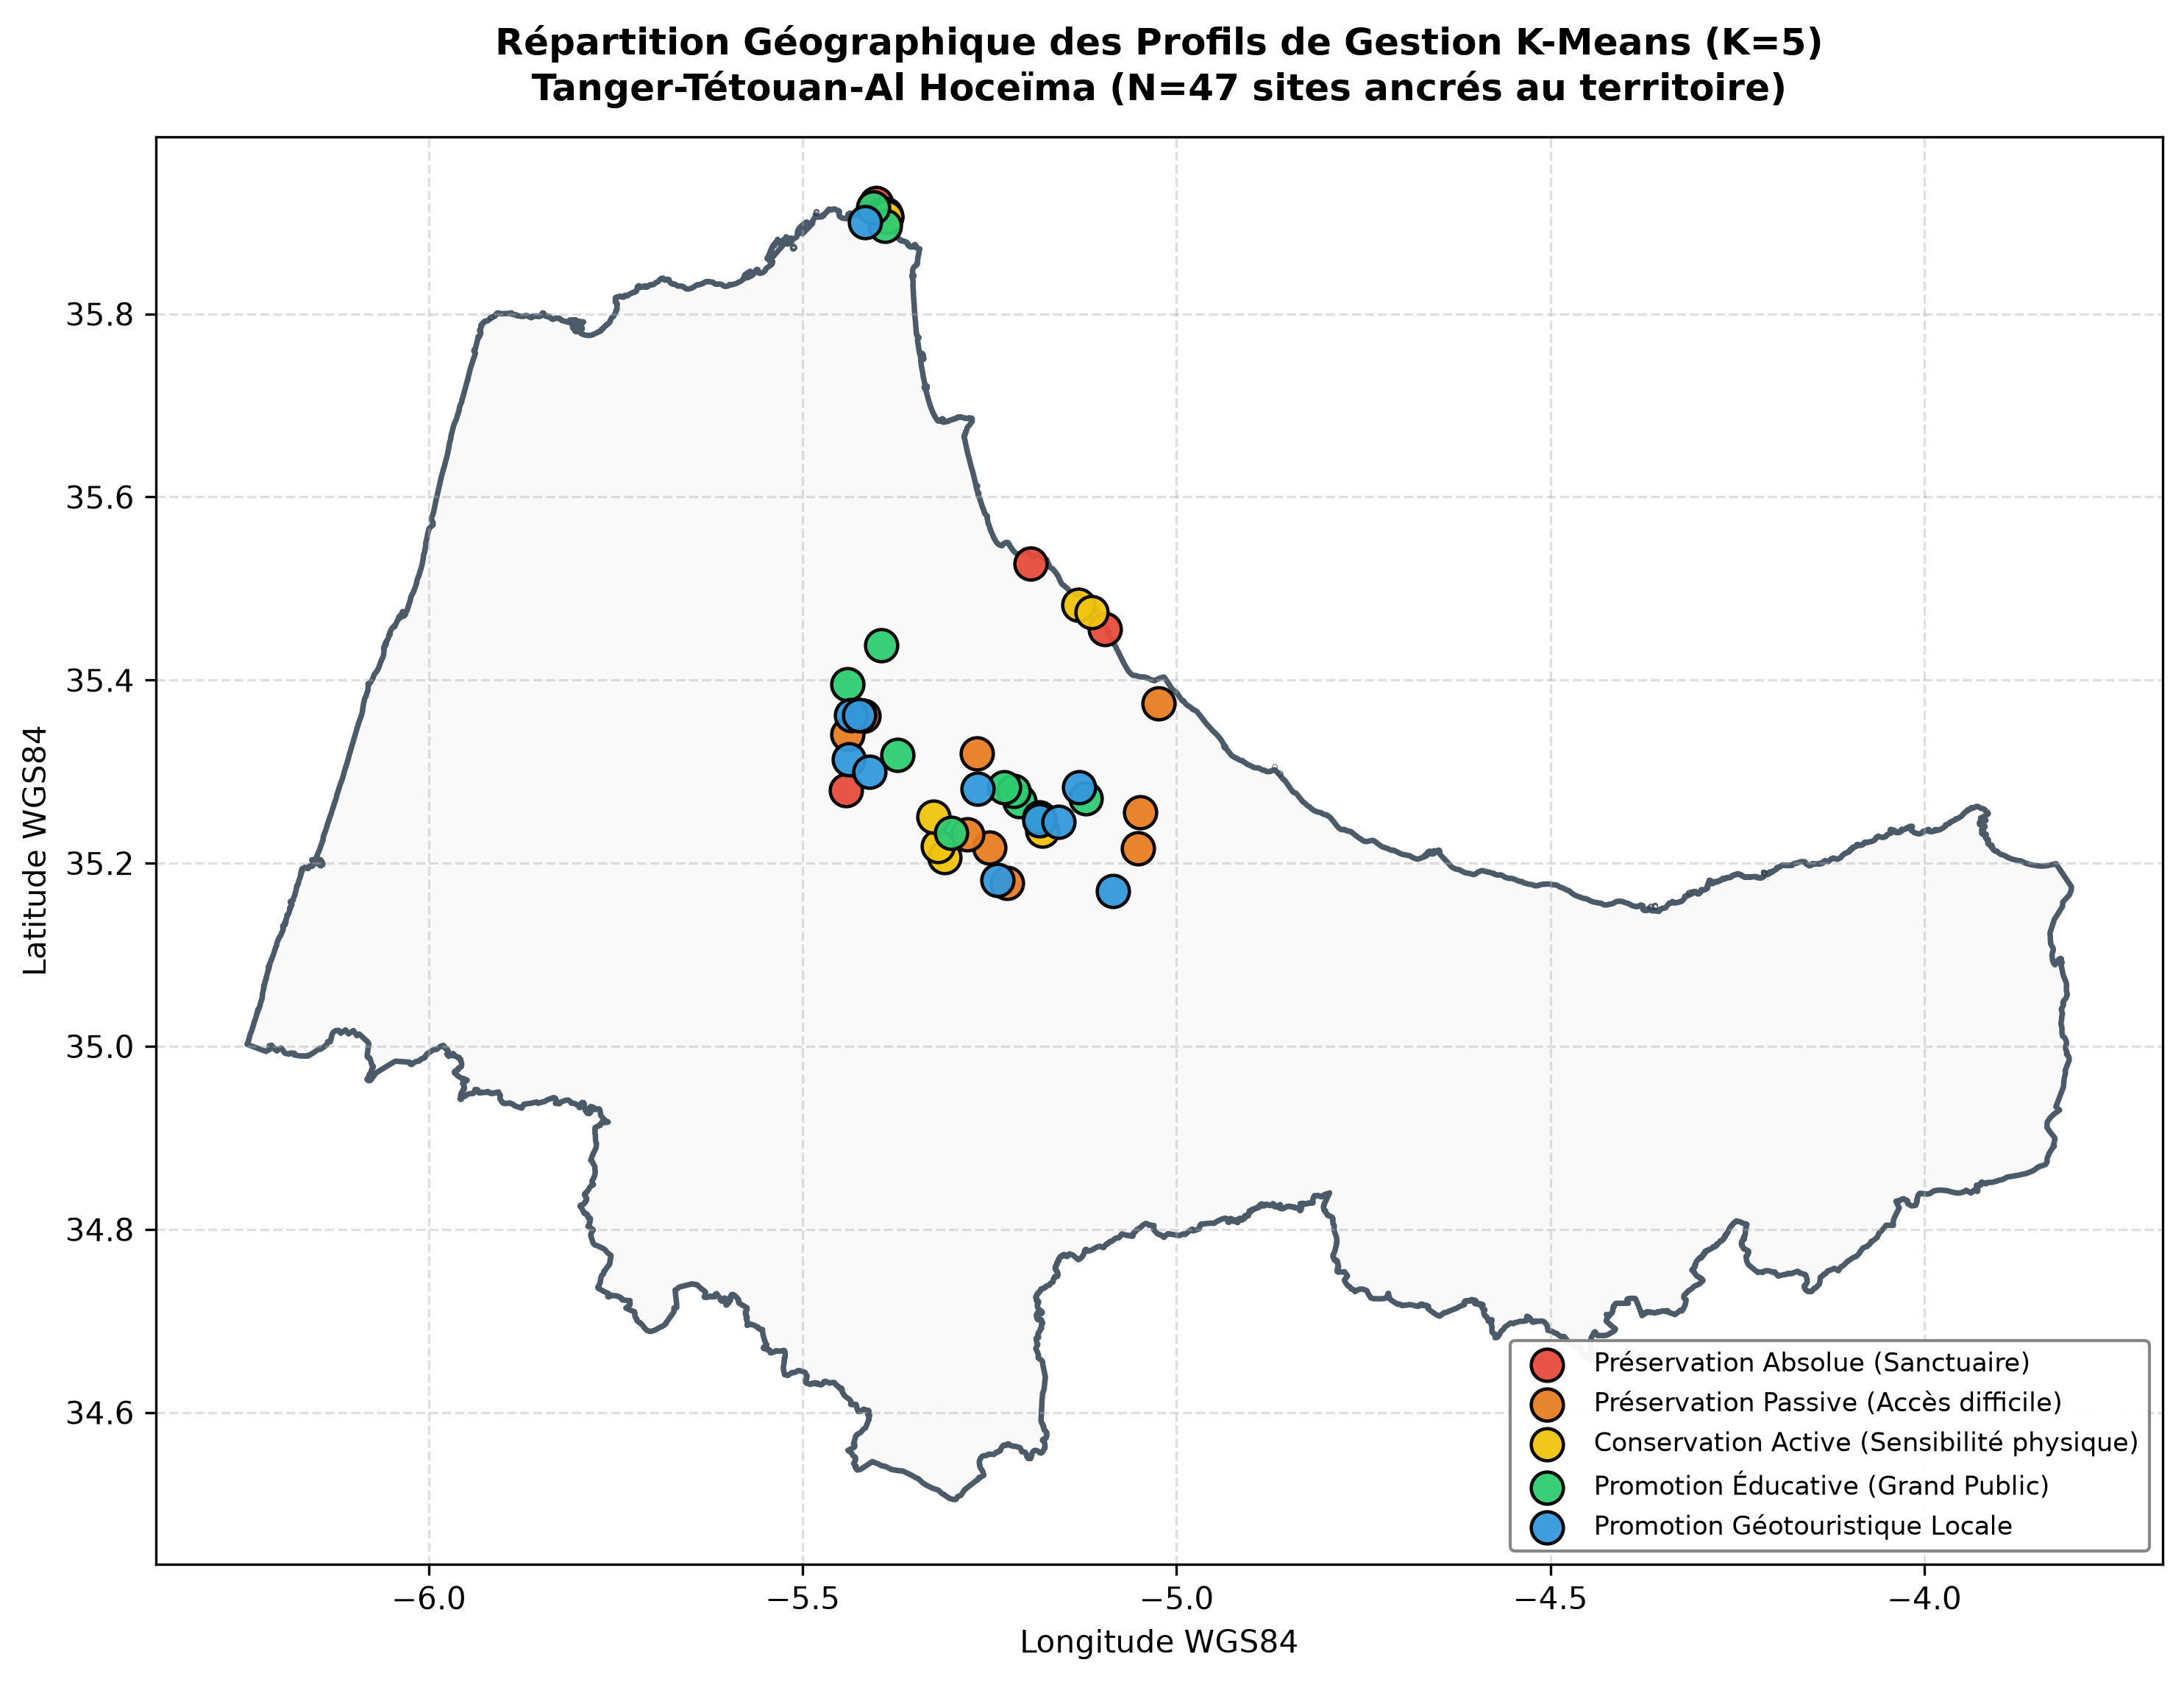
\includegraphics[width=\linewidth]{../figures/ttah_geosites_spatial_clusters.png}
    \caption{Répartition géographique des profils de gestion K-Means pour la région Tanger-Tétouan-Al Hoceïma ($N=47$ géosites strictement situés à l'intérieur du territoire provincial).}
    \label{fig:ttah_spat_clust}
\end{figure}

\subsection{Projections Cartographiques Régionales et Concordance}
Les modèles régionaux entraînés ont été projetés sur la grille raster physique de chaque région ($19\,585$ pixels terrestres pour BMK et $11\,544$ pixels pour TTAH).

La comparaison entre le modèle national flou et les modèles régionaux localisés (Figures \ref{fig:bmk_map} et \ref{fig:ttah_map}) démontre une \textbf{forte concordance spatiale} :
\begin{itemize}
    \item \textbf{Béni Mellal-Khénifra} : Concordance globale de \textbf{85,93\%} (16 829 pixels identiques sur 19 585).
    \item \textbf{Tanger-Tétouan-Al Hoceïma} : Concordance globale de \textbf{89,32\%} (10 311 pixels identiques sur 11 544).
\end{itemize}

\begin{figure*}[htbp]
    \centering
    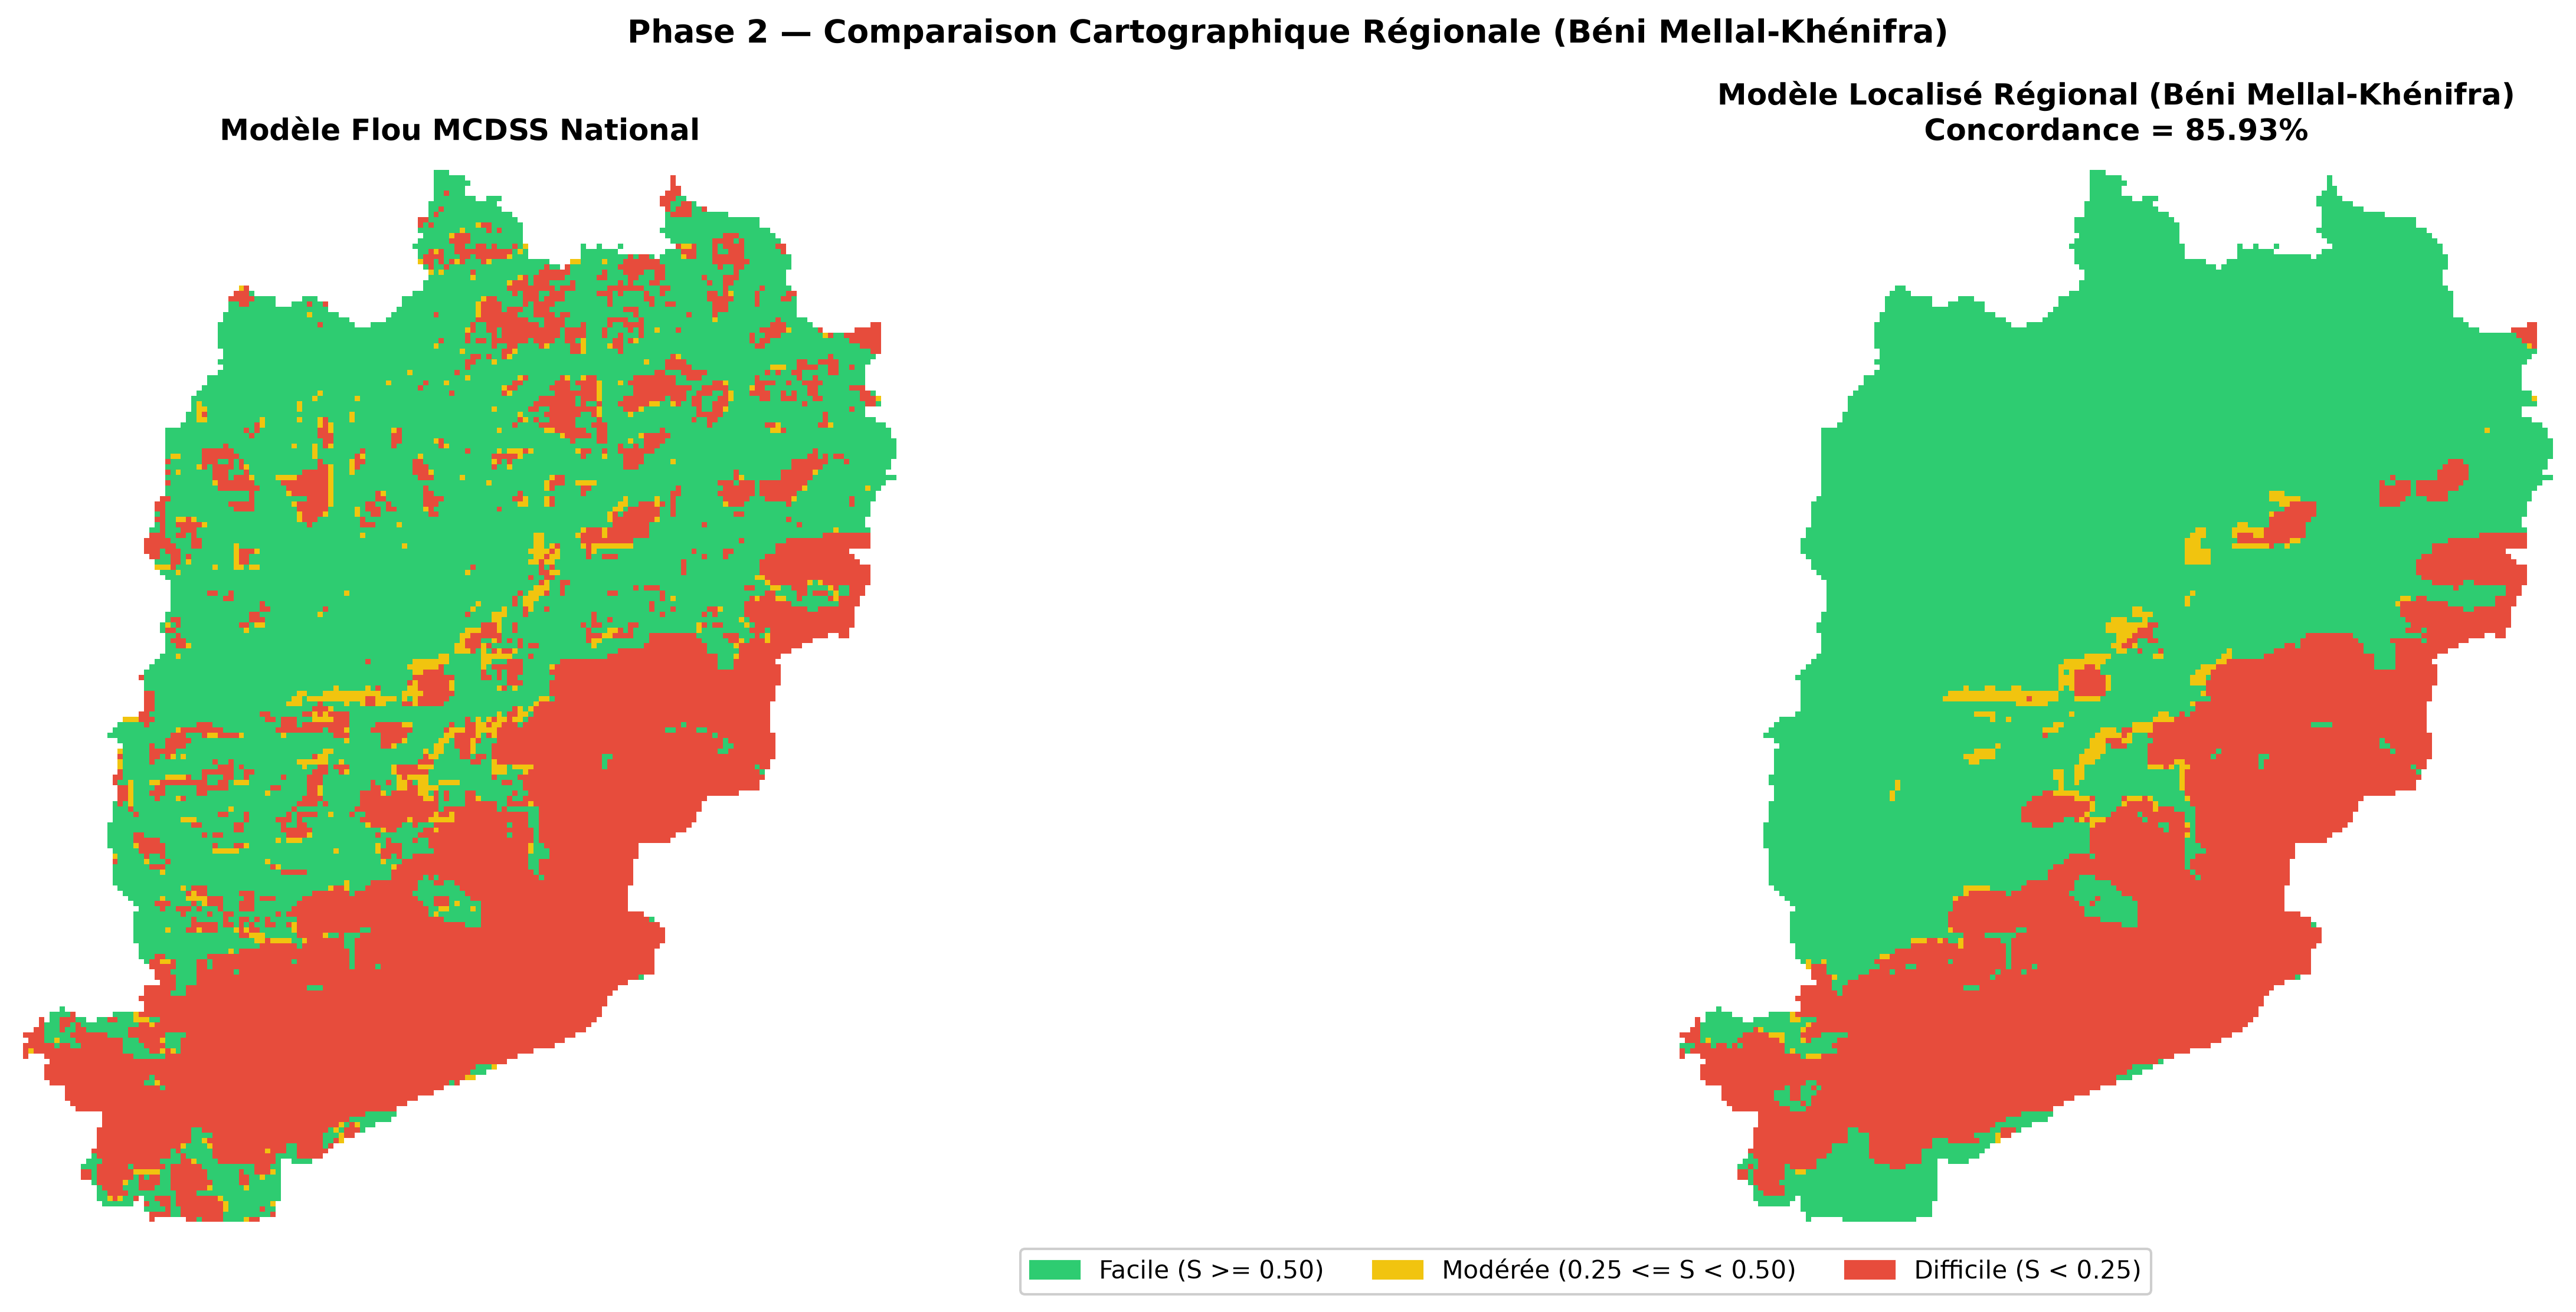
\includegraphics[width=0.95\linewidth]{../figures/comparative_accessibility_grid_map.png}
    \caption{Comparaison des projections raster pour Béni Mellal-Khénifra : Modèle National Flou (gauche) vs. Modèle Régional Localisé (droite). Le repère (1) localise le secteur du plateau Oulmès/Khouribga reclassé de Difficile à Facile.}
    \label{fig:bmk_map}
\end{figure*}

\begin{figure*}[htbp]
    \centering
    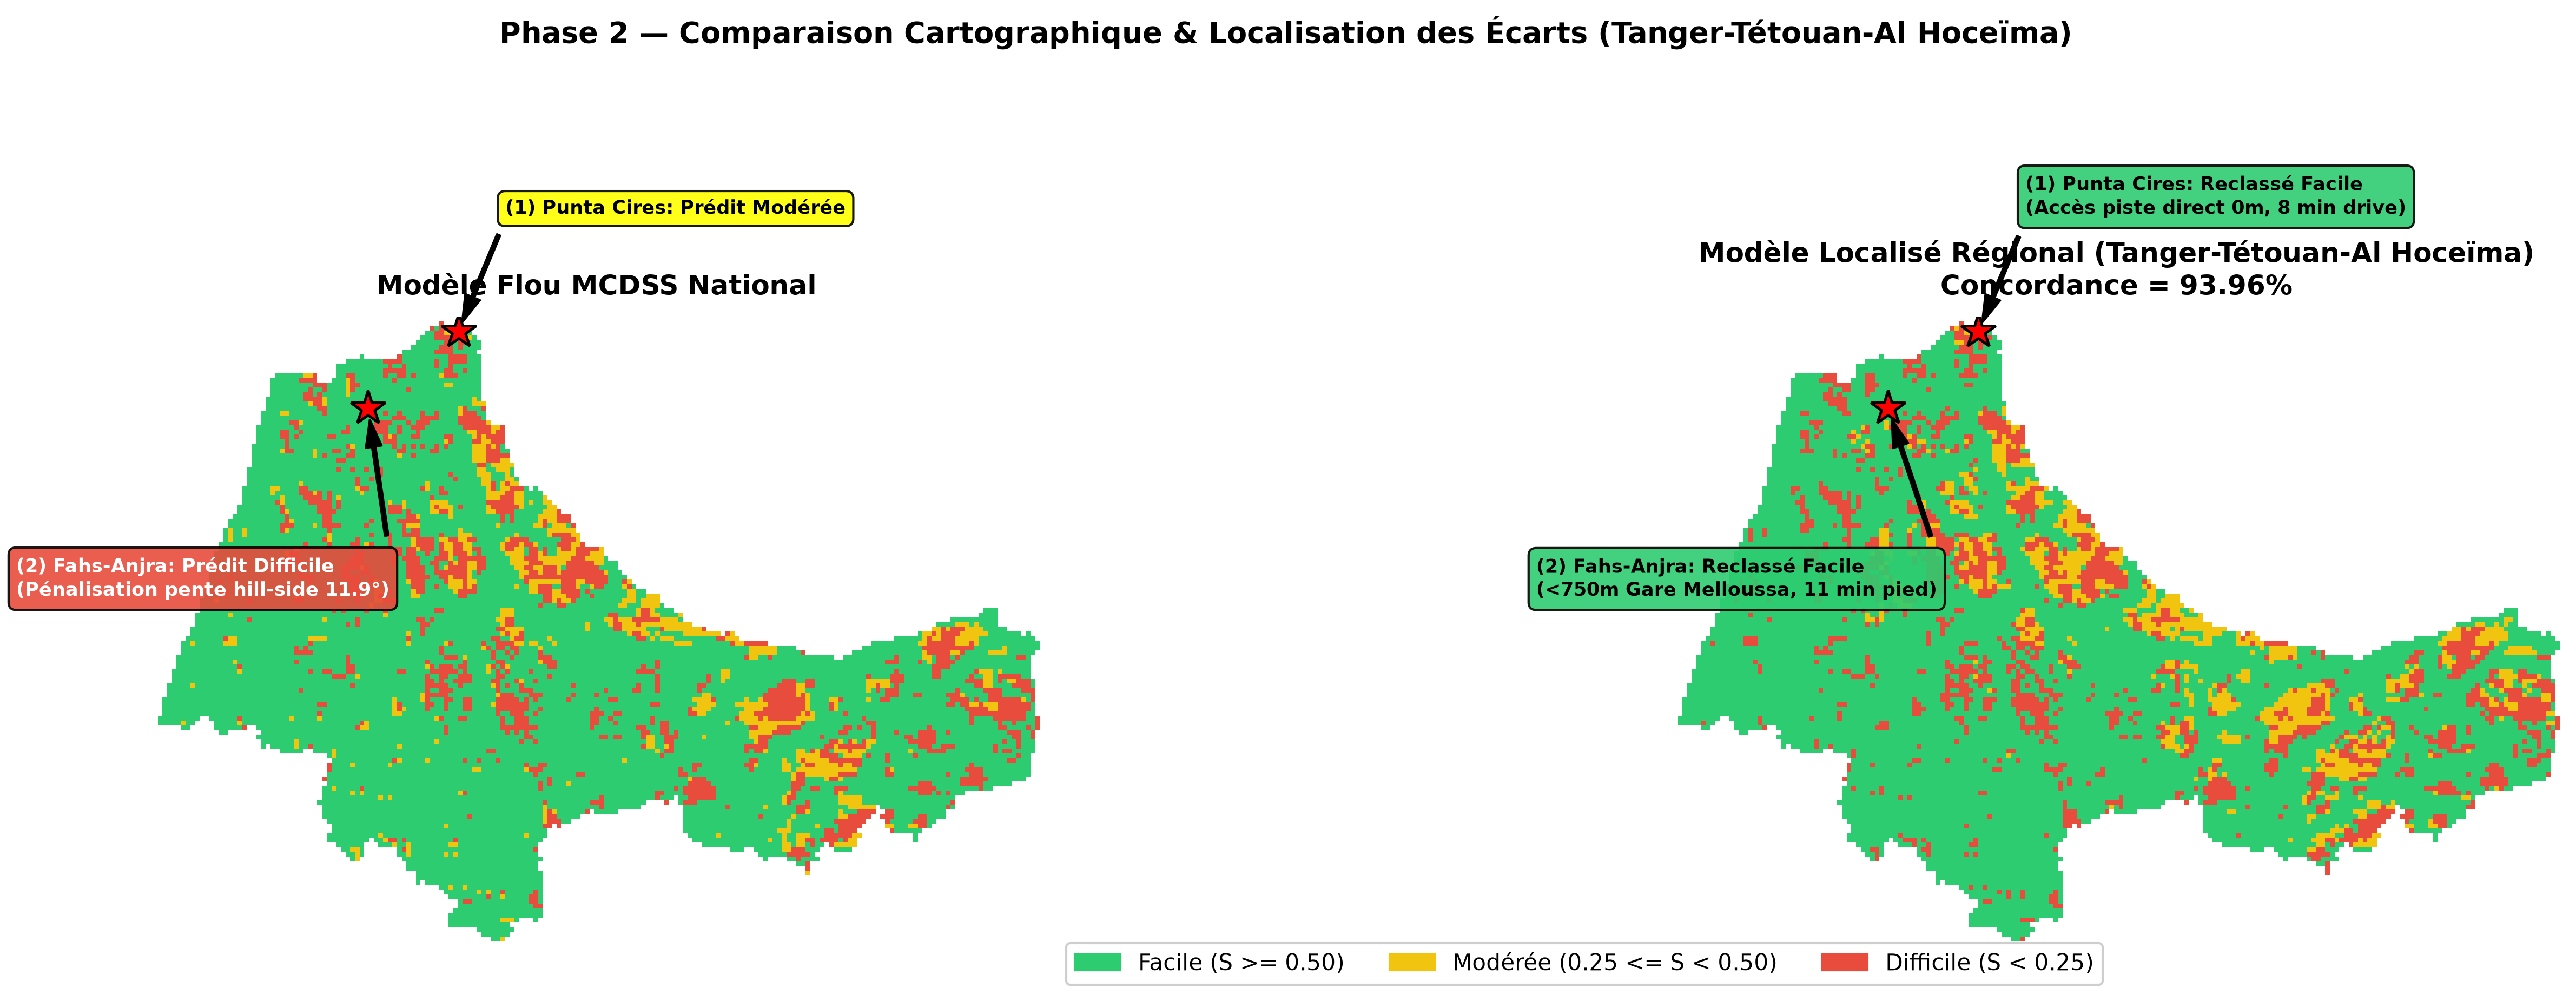
\includegraphics[width=0.95\linewidth]{../figures/ttah_comparative_grid_map.png}
    \caption{Comparaison des projections raster pour Tanger-Tétouan-Al Hoceïma : Modèle National Flou (gauche) vs. Modèle Régional Localisé (droite). Les repères (1) (Punta Cires) et (2) (Fahs-Anjra) mettent en évidence les zones de reclassification locale.}
    \label{fig:ttah_map}
\end{figure*}

\subsection{Analyse Micro-Topographique des Écarts Prédictifs}
L'inspection détaillée des repères cartographiques (Figures \ref{fig:bmk_map} et \ref{fig:ttah_map}) et la validation croisée par itinéraire Google Maps révèlent que les modèles régionaux apportent un gain de réalisme territorial significatif en corrigeant les sur-pénalisations du modèle national macroscopique :

\begin{enumerate}
    \item \textbf{Validation de Terrain Périurbain (Collines de Fahs-Anjra, Repère (2), Figures \ref{fig:ttah_map} et \ref{fig:melloussa})} : Au point ($35,7250^\circ\,\text{N}, -5,6685^\circ\,\text{W}$), le modèle national classait la zone en \textbf{Difficile} en raison de la pente hill-side ($11,9^\circ$). La vérification par itinéraire confirme que le site est situé à moins de \textbf{750\,m (11 min à pied)} de la \textbf{Gare de Melloussa} (Figure \ref{fig:melloussa}). Le modèle régional TTAH reclassifie avec succès cette zone en \textbf{Facile}, capturant la haute accessibilité multimodale périurbaine.
    \item \textbf{Reclassification et Logistique d'Accès (Punta Cires, Repère (1), Figure \ref{fig:ttah_map})} : Pour le géosite \emph{The flute casts of Punta Cires} ($35,9000^\circ\,\text{N}, -5,4167^\circ\,\text{W}$), le modèle national prédisait \textbf{Modérée} à cause de la rugosité régionale du Rif ($R=263,5$). L'analyse d'itinéraire depuis Belyounech vers la forêt de Jbel Moussa indique un trajet véhicule de seulement \textbf{8 min (2,7 km)} via les pistes, contre un itinéraire pédestre de \textbf{1h 05min (4,1 km, $+212\,\text{m}$ de dénivelé)}. Le modèle régional localisé saisit avec précision l'accessibilité routière directe par piste ($0\,\text{m}$), reclassant le site en \textbf{Facile}.
    \item \textbf{Nuance sur Grille BMK (Plateau Oulmès/Khouribga, Repère (1), Figure \ref{fig:bmk_map})} : Au point ($33,4720^\circ\,\text{N}, -6,9462^\circ\,\text{W}$), le modèle national prédisait \textbf{Difficile} (éloignement des axes principaux $>3,5\,\text{km}$). Le modèle régional BMK réévalue le pixel en \textbf{Facile} du fait de la topographie quasi-plane ($\theta=1,8^\circ, R=50,4$). Cependant, l'analyse d'accès indique que sans voie goudronnée à proximité, ce reclassement constitue une surestimation de l'accessibilité pédestre en zone rurale isolée.
\end{enumerate}

\begin{figure}[htbp]
    \centering
    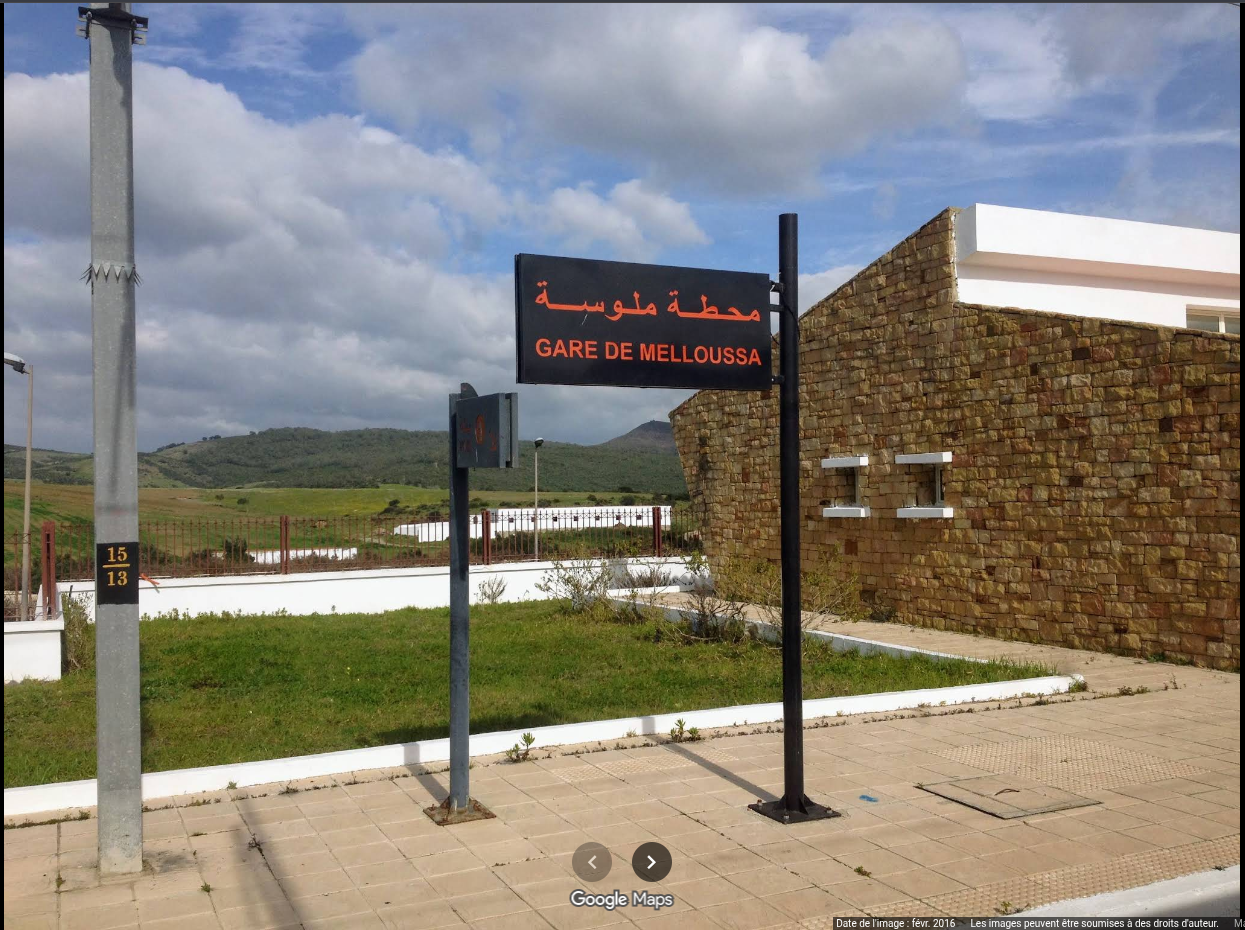
\includegraphics[width=\linewidth]{../figures/Mellousa_Fahs-Anjra_Coastal_Hills.png}
    \caption{Preuve d'infrastructure de transport : La Gare de Melloussa (Tanger-Tétouan-Al Hoceïma), située à moins de 750 m (<11 min à pied) du secteur de Fahs-Anjra (Repère (2)), justifiant la reclassification en accessibilité Facile par le modèle régional localisé.}
    \label{fig:melloussa}
\end{figure}

\section{Conclusions et Perspectives Régionales}
Le déploiement du moteur \textbf{Fuzzy MCDSS} en Phase 2 confirme la stabilité et la haute concordance (\textbf{85,93\%} à \textbf{89,32\%}) des prédictions pré-établies tout en offrant une finesse d'analyse territoriale indispensable pour la gestion opérationnelle du géopatrimoine régional. La combinaison du découpage flou et du clustering K-Means ($K=5$) fournit aux décisionnaires de l'UM6P et des conseils régionaux un outil rigoureux pour orienter les investissements en géotourisme durable et en conservation du patrimoine naturel.

\section*{Remerciements}
Nous remercions le Geology and Sustainable Mining Institute (GSMI) et l'Université Mohammed VI Polytechnique (UM6P) pour leur soutien constant.

\begin{thebibliography}{1}
\bibitem{brilha2016}
J. Brilha, ``Inventory and Quantitative Assessment of Geosites and Geodiversity Sites: a Review,'' \emph{Geoheritage}, vol. 8, n\textsuperscript{o} 2, pp. 119--134, 2016.
\bibitem{naimi2025}
M. Manaouch, L. Naimi, M. Haynou, M. Aghad, M. Sadiki, Q. B. Pham et A. Jakimi, ``Enhancing Geotourism in Southeastern Morocco through Machine Learning-Based Geomorphosite Identification,'' \emph{Geoheritage}, vol. 17, n\textsuperscript{o} 34, 2025.
\end{thebibliography}

\end{document}
